% Options for packages loaded elsewhere
\PassOptionsToPackage{unicode}{hyperref}
\PassOptionsToPackage{hyphens}{url}
%
\documentclass[
  ignorenonframetext,
]{beamer}
\usepackage{pgfpages}
\setbeamertemplate{caption}[numbered]
\setbeamertemplate{caption label separator}{: }
\setbeamercolor{caption name}{fg=normal text.fg}
\beamertemplatenavigationsymbolsempty
% Prevent slide breaks in the middle of a paragraph
\widowpenalties 1 10000
\raggedbottom
\setbeamertemplate{part page}{
  \centering
  \begin{beamercolorbox}[sep=16pt,center]{part title}
    \usebeamerfont{part title}\insertpart\par
  \end{beamercolorbox}
}
\setbeamertemplate{section page}{
  \centering
  \begin{beamercolorbox}[sep=12pt,center]{part title}
    \usebeamerfont{section title}\insertsection\par
  \end{beamercolorbox}
}
\setbeamertemplate{subsection page}{
  \centering
  \begin{beamercolorbox}[sep=8pt,center]{part title}
    \usebeamerfont{subsection title}\insertsubsection\par
  \end{beamercolorbox}
}
\AtBeginPart{
  \frame{\partpage}
}
\AtBeginSection{
  \ifbibliography
  \else
    \frame{\sectionpage}
  \fi
}
\AtBeginSubsection{
  \frame{\subsectionpage}
}

\usepackage{amsmath,amssymb}
\usepackage{iftex}
\ifPDFTeX
  \usepackage[T1]{fontenc}
  \usepackage[utf8]{inputenc}
  \usepackage{textcomp} % provide euro and other symbols
\else % if luatex or xetex
  \usepackage{unicode-math}
  \defaultfontfeatures{Scale=MatchLowercase}
  \defaultfontfeatures[\rmfamily]{Ligatures=TeX,Scale=1}
\fi
\usepackage{lmodern}
\ifPDFTeX\else  
    % xetex/luatex font selection
\fi
% Use upquote if available, for straight quotes in verbatim environments
\IfFileExists{upquote.sty}{\usepackage{upquote}}{}
\IfFileExists{microtype.sty}{% use microtype if available
  \usepackage[]{microtype}
  \UseMicrotypeSet[protrusion]{basicmath} % disable protrusion for tt fonts
}{}
\makeatletter
\@ifundefined{KOMAClassName}{% if non-KOMA class
  \IfFileExists{parskip.sty}{%
    \usepackage{parskip}
  }{% else
    \setlength{\parindent}{0pt}
    \setlength{\parskip}{6pt plus 2pt minus 1pt}}
}{% if KOMA class
  \KOMAoptions{parskip=half}}
\makeatother
\usepackage{xcolor}
\newif\ifbibliography
\setlength{\emergencystretch}{3em} % prevent overfull lines
\setcounter{secnumdepth}{-\maxdimen} % remove section numbering


\providecommand{\tightlist}{%
  \setlength{\itemsep}{0pt}\setlength{\parskip}{0pt}}\usepackage{longtable,booktabs,array}
\usepackage{calc} % for calculating minipage widths
\usepackage{caption}
% Make caption package work with longtable
\makeatletter
\def\fnum@table{\tablename~\thetable}
\makeatother
\usepackage{graphicx}
\makeatletter
\def\maxwidth{\ifdim\Gin@nat@width>\linewidth\linewidth\else\Gin@nat@width\fi}
\def\maxheight{\ifdim\Gin@nat@height>\textheight\textheight\else\Gin@nat@height\fi}
\makeatother
% Scale images if necessary, so that they will not overflow the page
% margins by default, and it is still possible to overwrite the defaults
% using explicit options in \includegraphics[width, height, ...]{}
\setkeys{Gin}{width=\maxwidth,height=\maxheight,keepaspectratio}
% Set default figure placement to htbp
\makeatletter
\def\fps@figure{htbp}
\makeatother
% definitions for citeproc citations
\NewDocumentCommand\citeproctext{}{}
\NewDocumentCommand\citeproc{mm}{%
  \begingroup\def\citeproctext{#2}\cite{#1}\endgroup}
\makeatletter
 % allow citations to break across lines
 \let\@cite@ofmt\@firstofone
 % avoid brackets around text for \cite:
 \def\@biblabel#1{}
 \def\@cite#1#2{{#1\if@tempswa , #2\fi}}
\makeatother
\newlength{\cslhangindent}
\setlength{\cslhangindent}{1.5em}
\newlength{\csllabelwidth}
\setlength{\csllabelwidth}{3em}
\newenvironment{CSLReferences}[2] % #1 hanging-indent, #2 entry-spacing
 {\begin{list}{}{%
  \setlength{\itemindent}{0pt}
  \setlength{\leftmargin}{0pt}
  \setlength{\parsep}{0pt}
  % turn on hanging indent if param 1 is 1
  \ifodd #1
   \setlength{\leftmargin}{\cslhangindent}
   \setlength{\itemindent}{-1\cslhangindent}
  \fi
  % set entry spacing
  \setlength{\itemsep}{#2\baselineskip}}}
 {\end{list}}
\usepackage{calc}
\newcommand{\CSLBlock}[1]{\hfill\break\parbox[t]{\linewidth}{\strut\ignorespaces#1\strut}}
\newcommand{\CSLLeftMargin}[1]{\parbox[t]{\csllabelwidth}{\strut#1\strut}}
\newcommand{\CSLRightInline}[1]{\parbox[t]{\linewidth - \csllabelwidth}{\strut#1\strut}}
\newcommand{\CSLIndent}[1]{\hspace{\cslhangindent}#1}

\makeatletter
\@ifpackageloaded{caption}{}{\usepackage{caption}}
\AtBeginDocument{%
\ifdefined\contentsname
  \renewcommand*\contentsname{Table of contents}
\else
  \newcommand\contentsname{Table of contents}
\fi
\ifdefined\listfigurename
  \renewcommand*\listfigurename{List of Figures}
\else
  \newcommand\listfigurename{List of Figures}
\fi
\ifdefined\listtablename
  \renewcommand*\listtablename{List of Tables}
\else
  \newcommand\listtablename{List of Tables}
\fi
\ifdefined\figurename
  \renewcommand*\figurename{Figure}
\else
  \newcommand\figurename{Figure}
\fi
\ifdefined\tablename
  \renewcommand*\tablename{Table}
\else
  \newcommand\tablename{Table}
\fi
}
\@ifpackageloaded{float}{}{\usepackage{float}}
\floatstyle{ruled}
\@ifundefined{c@chapter}{\newfloat{codelisting}{h}{lop}}{\newfloat{codelisting}{h}{lop}[chapter]}
\floatname{codelisting}{Listing}
\newcommand*\listoflistings{\listof{codelisting}{List of Listings}}
\makeatother
\makeatletter
\makeatother
\makeatletter
\@ifpackageloaded{caption}{}{\usepackage{caption}}
\@ifpackageloaded{subcaption}{}{\usepackage{subcaption}}
\makeatother
\ifLuaTeX
  \usepackage{selnolig}  % disable illegal ligatures
\fi
\IfFileExists{bookmark.sty}{\usepackage{bookmark}}{\usepackage{hyperref}}
\IfFileExists{xurl.sty}{\usepackage{xurl}}{} % add URL line breaks if available
\urlstyle{same} % disable monospaced font for URLs
\hypersetup{
  pdftitle={Heavy-snow transform},
  pdfauthor={Guebin Choi},
  hidelinks,
  pdfcreator={LaTeX via pandoc}}

\title{Heavy-snow transform}
\subtitle{A new multiscale method for non-Euclidean data}
\author{Guebin Choi}
\date{}

\begin{document}
\frame{\titlepage}

\begin{frame}{Contents}
\phantomsection\label{contents}
\begin{itemize}
\item
  Motivation
\item
  Proposed method (quick view)
\item
  Related studies
\item
  Proposed method
\item
  Real data analysis
\end{itemize}
\end{frame}

\begin{frame}{Motivation}
\phantomsection\label{motivation}
\begin{block}{Non-Euclidean data}
\phantomsection\label{non-euclidean-data}
\begin{itemize}
\item
  Non-Euclidean data is data that cannot be stored in a grid or array
  form, such as graph and manifold data.
\item
  Specific examples of non-Euclidean data include 3D point cloud, gene
  expression, social network, and traffic data.

  \begin{itemize}
  \tightlist
  \item
    Euclidean data: time-series, audio, images \(\dots\)
  \item
    Non-Euclidean data: 3D point cloud data (manifold data), molecules,
    social networks \(\dots\)
  \end{itemize}
\end{itemize}
\end{block}
\end{frame}

\begin{frame}{Motivation}
\phantomsection\label{motivation-1}
\begin{block}{Graph Signal}
\begin{itemize}
\tightlist
\item
  Among non-Euclidean data, we consider a \textbf{graph signal}, which
  is a real-valued function whose domain is a graph or manifold.
\item
  Formally, the graph signal \(f\) is defined as a function such that
  \(f:{\cal V} \to \mathbb{R}\), where \({\cal V}\) is a set of nodes
  (or vertices). In here, \(f(v_i)\) and \(f(v_j)\) denote values at
  \(v_i\in {\cal V}\) and \(v_j\in {\cal V}\).
\end{itemize}
\end{block}

\begin{block}{Example: graph signal on Petersen graph}
\begin{figure}[H]

{\centering \includegraphics[width=0.5\textwidth,height=\textheight]{fig8_hst_graphsignal.png}

}

\caption{Fig1: A random positive graph signal on the vertices of the
Petersen graph. The height of each blue bar represent the signal value
at the vertex where the bar originates (Shuman et al. 2013).}

\end{figure}%
\end{block}
\end{frame}

\begin{frame}{Motivation}
\phantomsection\label{motivation-2}
How do we measure a similarity when there is a value on the manifold?

\begin{figure}[H]

{\centering 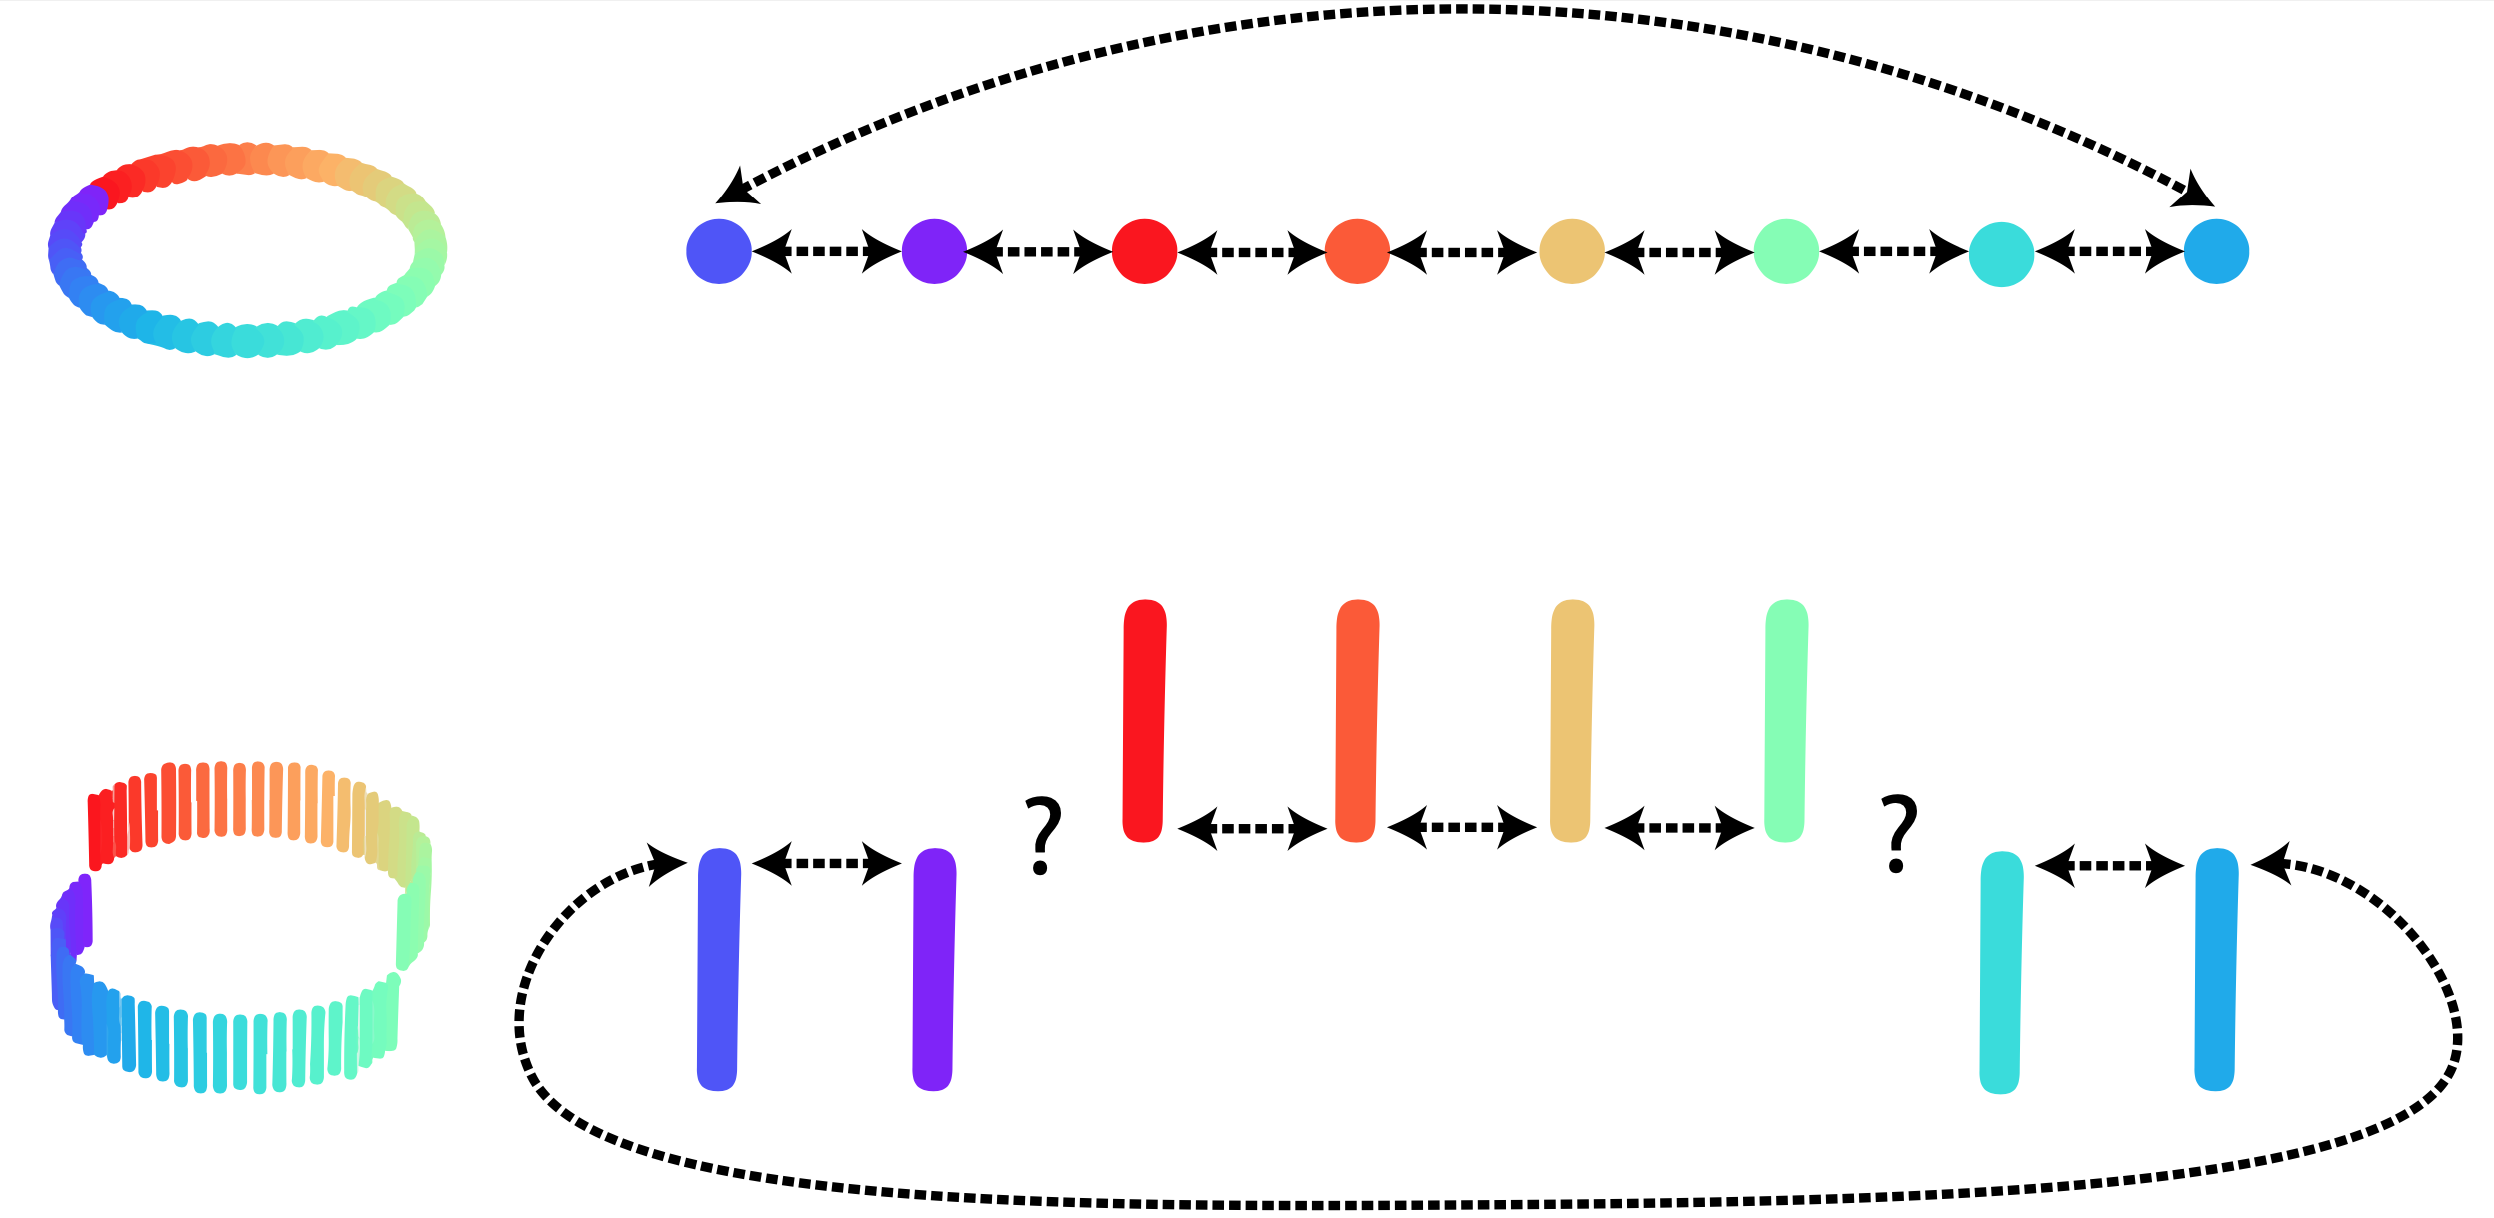
\includegraphics{Beamer_files/figure-beamer/bf181b9a-e50e-43ac-aa62-4f8c35b60cc0-1-740fdc07-677d-4d79-8f84-1506459bb231.png}

}

\caption{Fig2: The ring-shaped manifold (top) and ring-shaped manifold
with Euclidean values (bottom)}

\end{figure}%
\end{frame}

\begin{frame}{Motivation}
\phantomsection\label{motivation-3}
It is unclear which domain should we focus on, Euclid or graph?

\begin{figure}[H]

{\centering 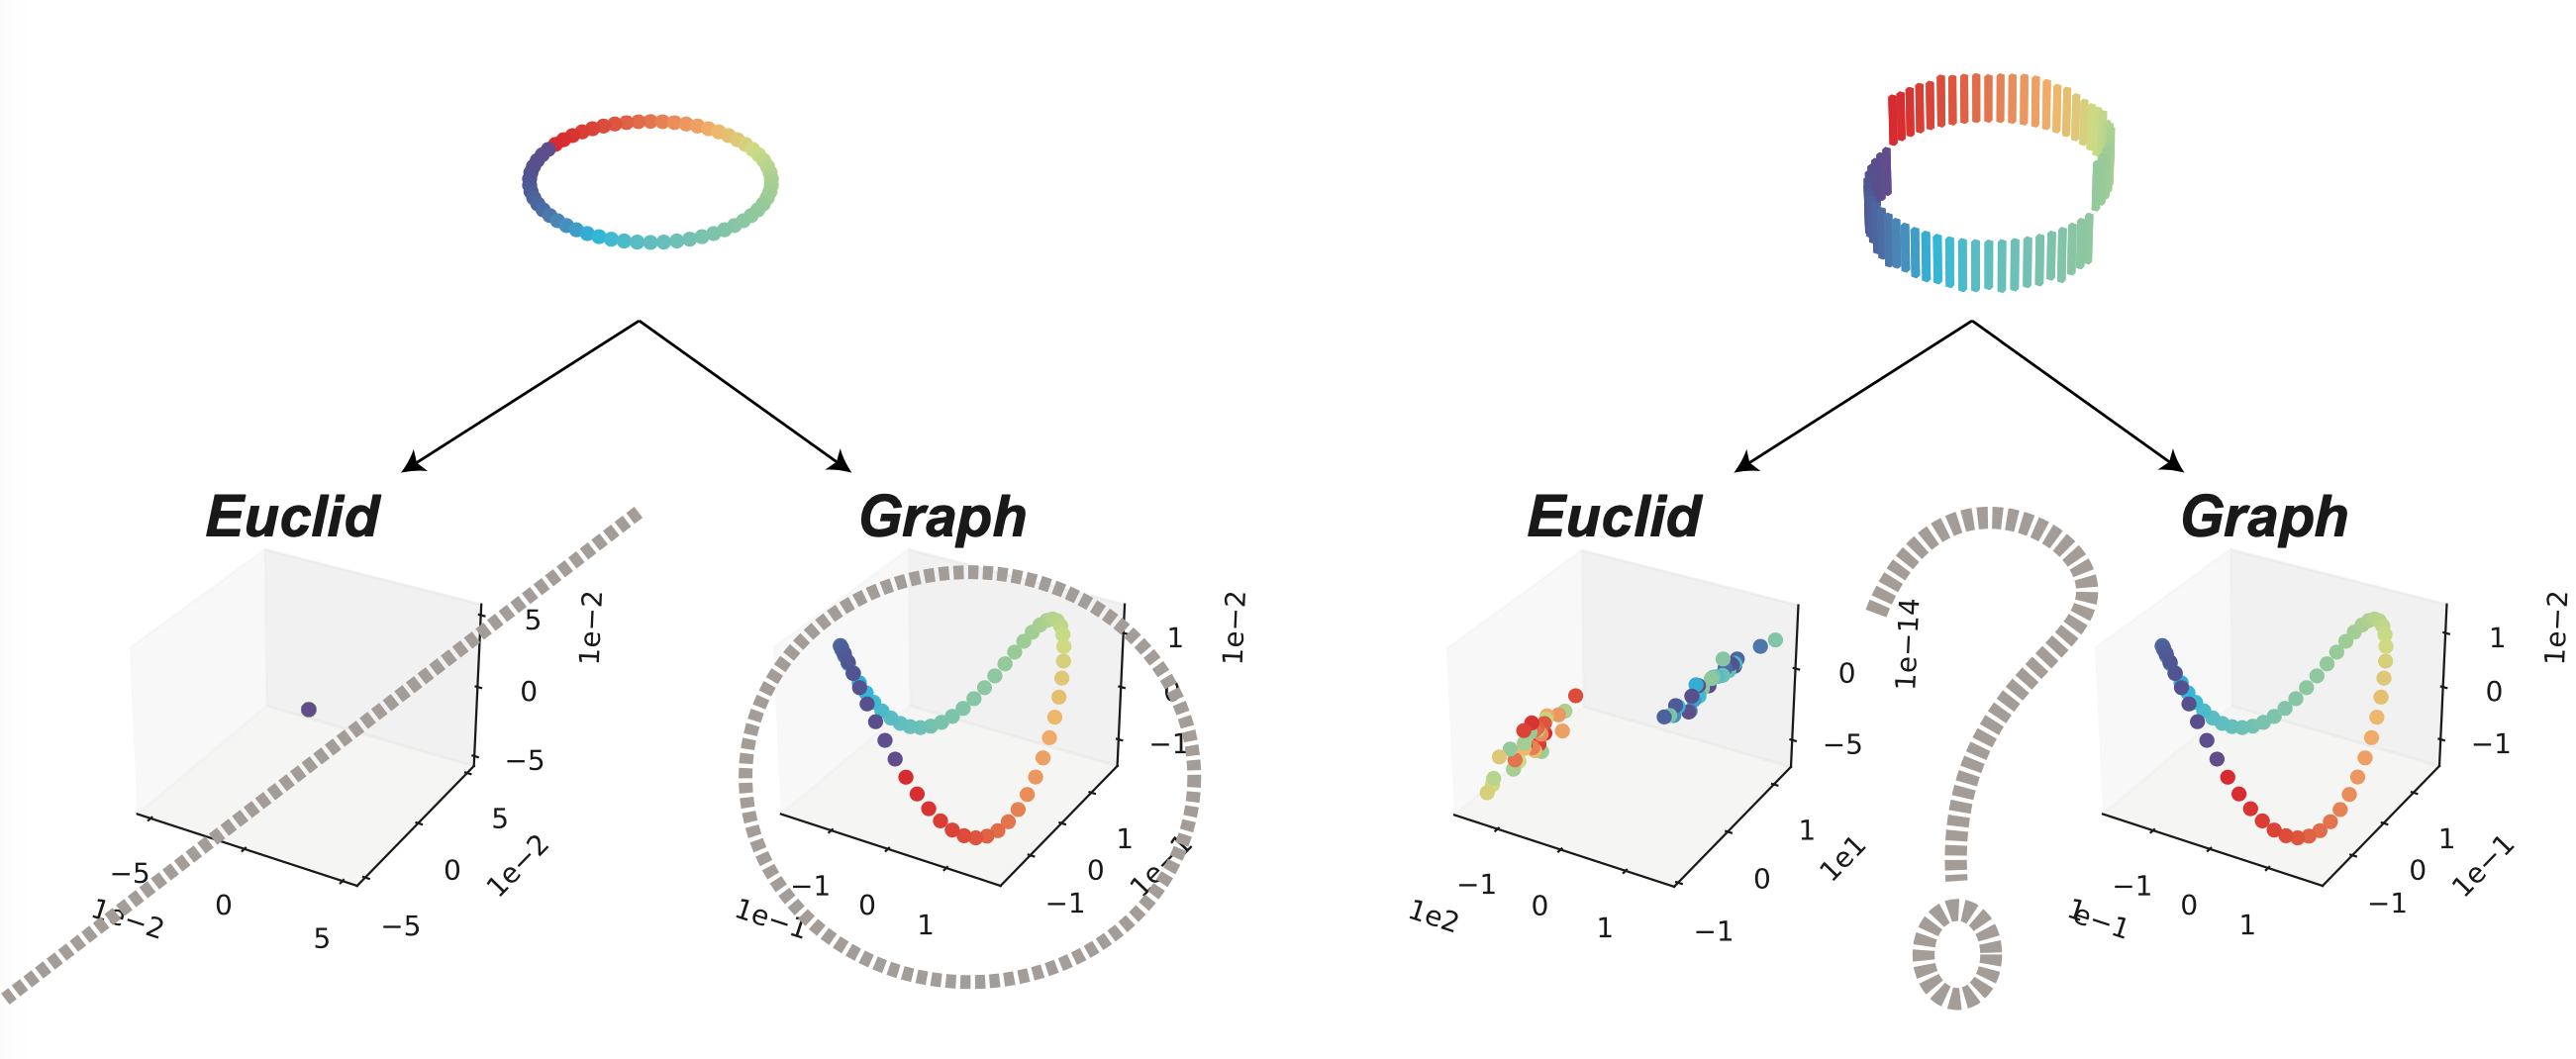
\includegraphics{Beamer_files/figure-beamer/792814a4-a462-4db9-accb-0adf18a1a0ce-1-20b92b21-f221-425c-83ca-7818c930841d.png}

}

\caption{Fig3: Two manifold data (top) and its embedding results
(bottom).}

\end{figure}%
\end{frame}

\begin{frame}{Motivation}
\phantomsection\label{motivation-4}
We want to consider the distances in both Euclidean and graph domains
simultaneously.

\begin{figure}[H]

{\centering 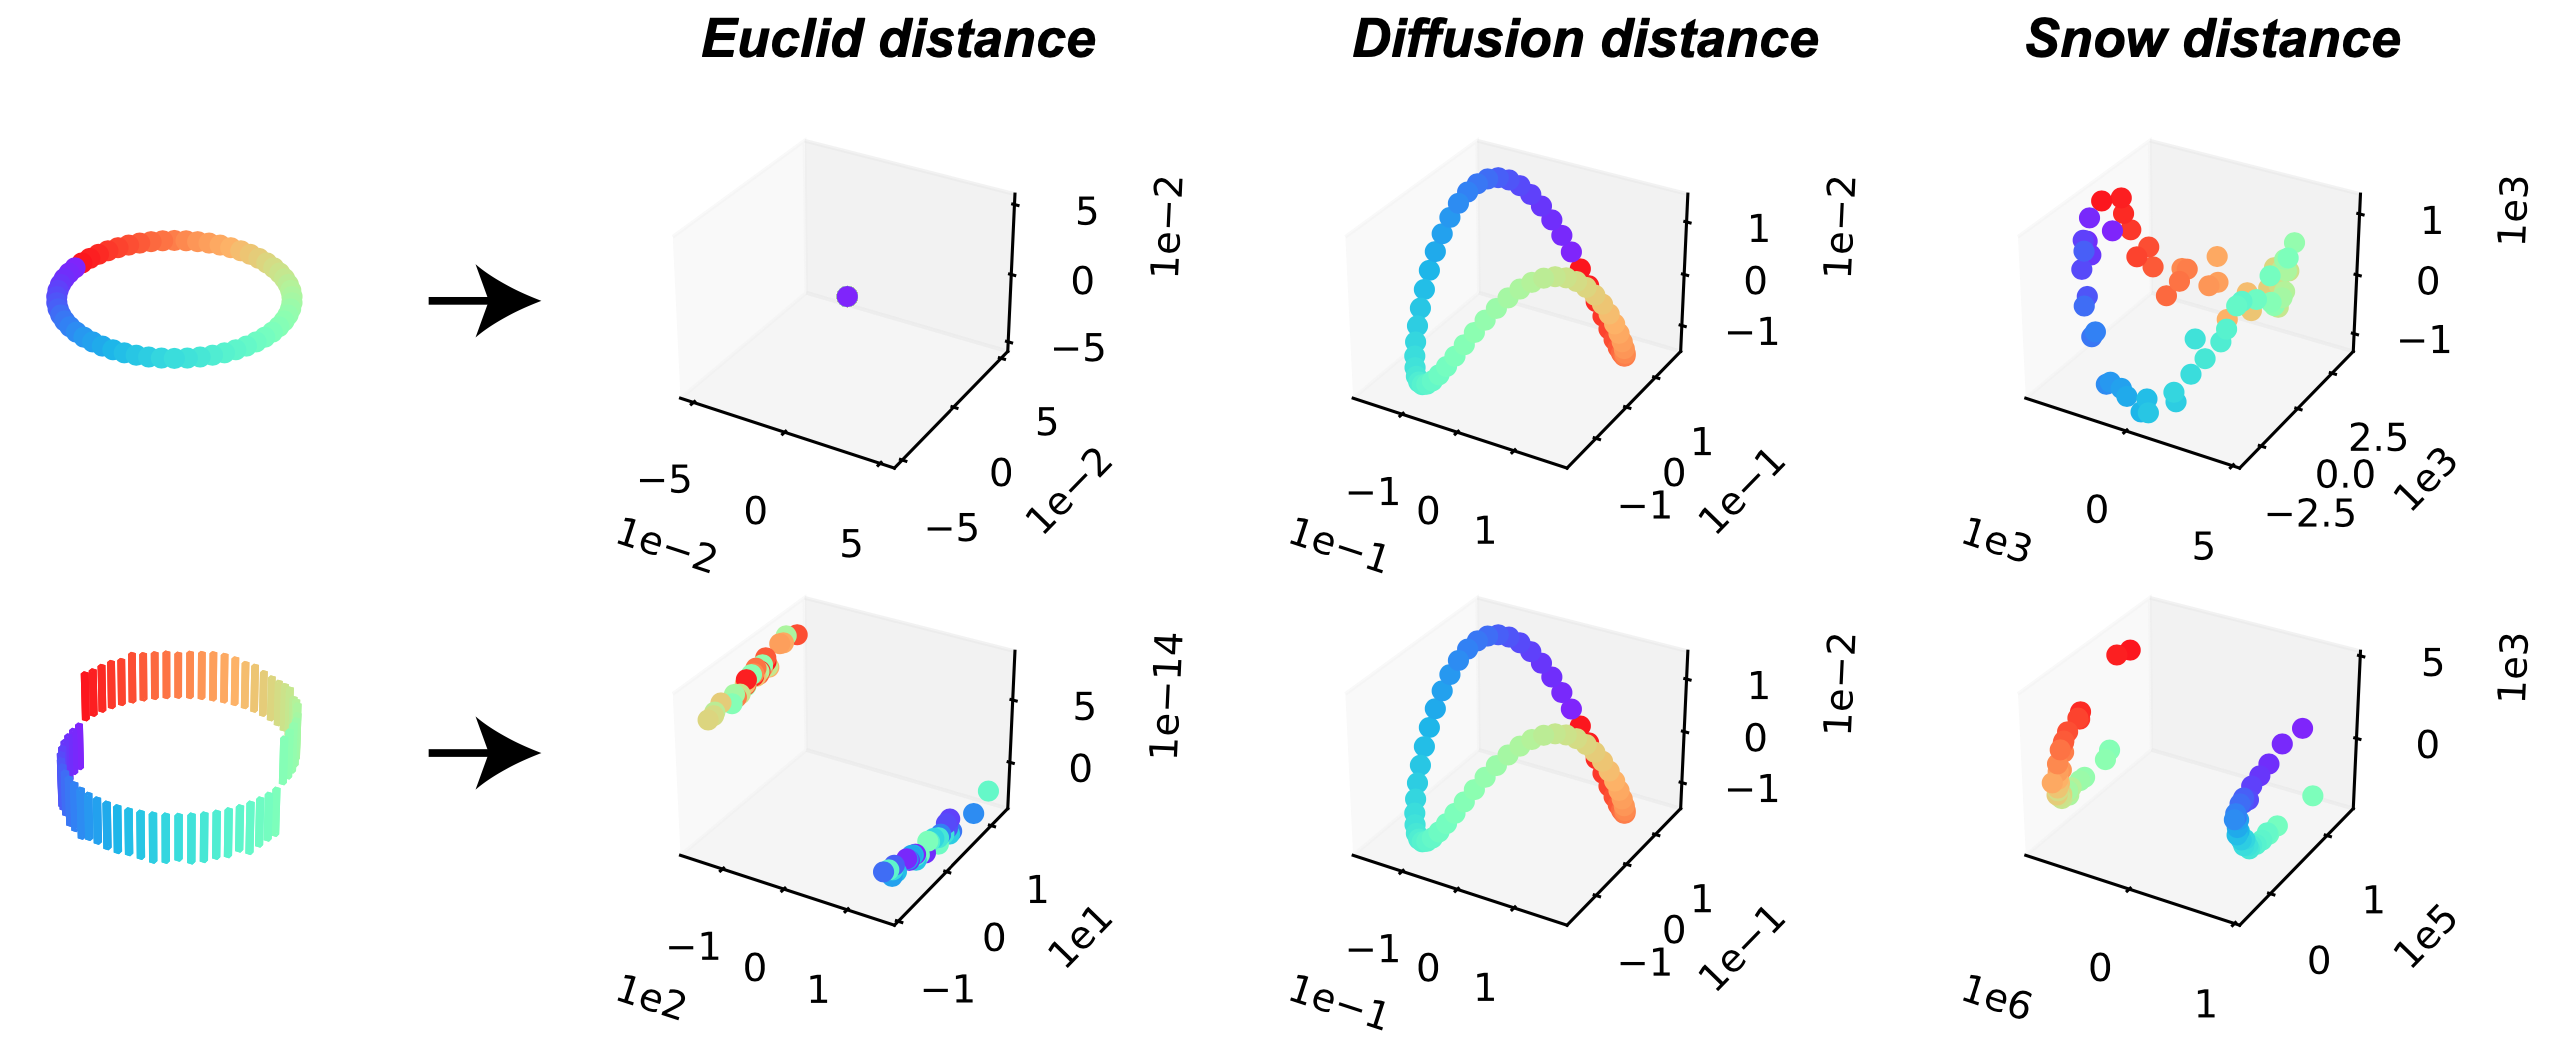
\includegraphics{Beamer_files/figure-beamer/d15df95f-ad86-4918-a938-24306749f03b-1-b961e7a3-ebb7-4ab0-95b6-84b604d7e9bc.png}

}

\caption{Fig4: Embedding results with three different distances.}

\end{figure}%
\end{frame}

\begin{frame}{Proposed method (quick view)}
\phantomsection\label{proposed-method-quick-view}
Before explaining the proposed method, let's consider the following
simple graph signal:

\begin{block}{Very simple Graph signal}
\begin{itemize}
\tightlist
\item
  \({\cal V}=\{v_1,v_2,v_3,v_4\}\)
\item
  \({\cal E}=\{(v_1,v_2), (v_2,v_3), (v_2,v_4) \}\)
\item
  \(f(v_1)=3, f(v_2)=1, f(v_3)=4, f(v_4)=5\)
\end{itemize}
\end{block}

\begin{block}{Figure}
\begin{figure}[H]

{\centering 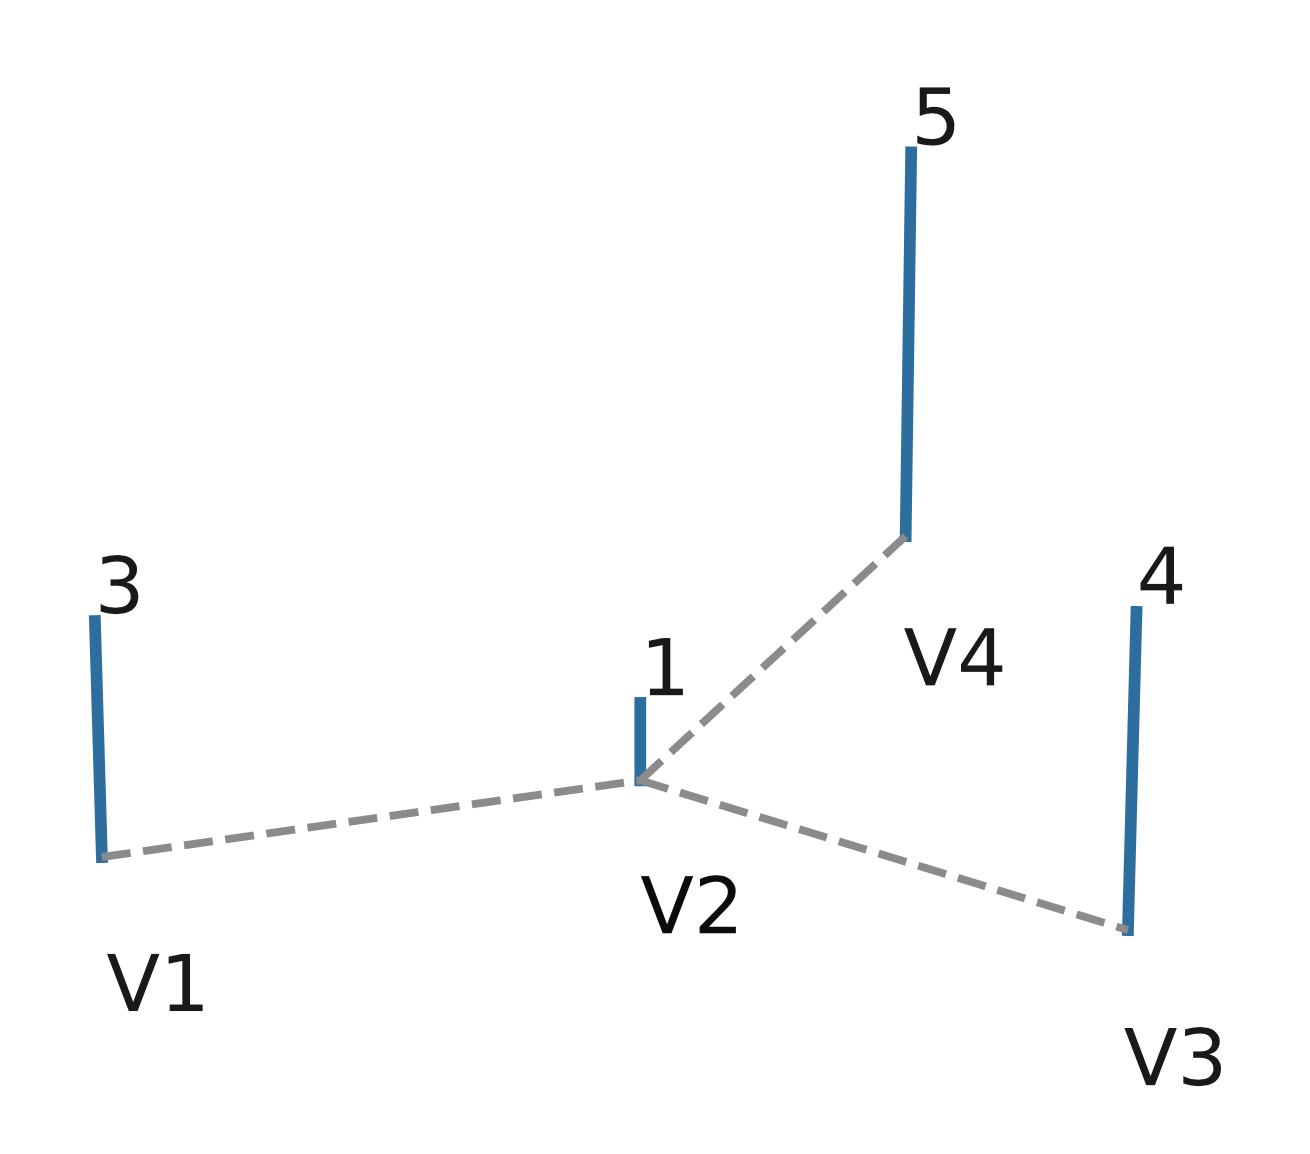
\includegraphics[width=0.3\textwidth,height=\textheight]{Beamer_files/figure-beamer/5fe2f6fb-8de3-4c35-b640-b4e436298018-1-a3fa2fbe-acea-4be6-8c44-c8781282a44f.png}

}

\caption{Fig5: The simple graph signal with 4 nodes.}

\end{figure}%
\end{block}
\end{frame}

\begin{frame}{Proposed method (quick view)}
\phantomsection\label{proposed-method-quick-view-1}
Distance matrix could be defined in the following two ways.

\begin{figure}[H]

{\centering 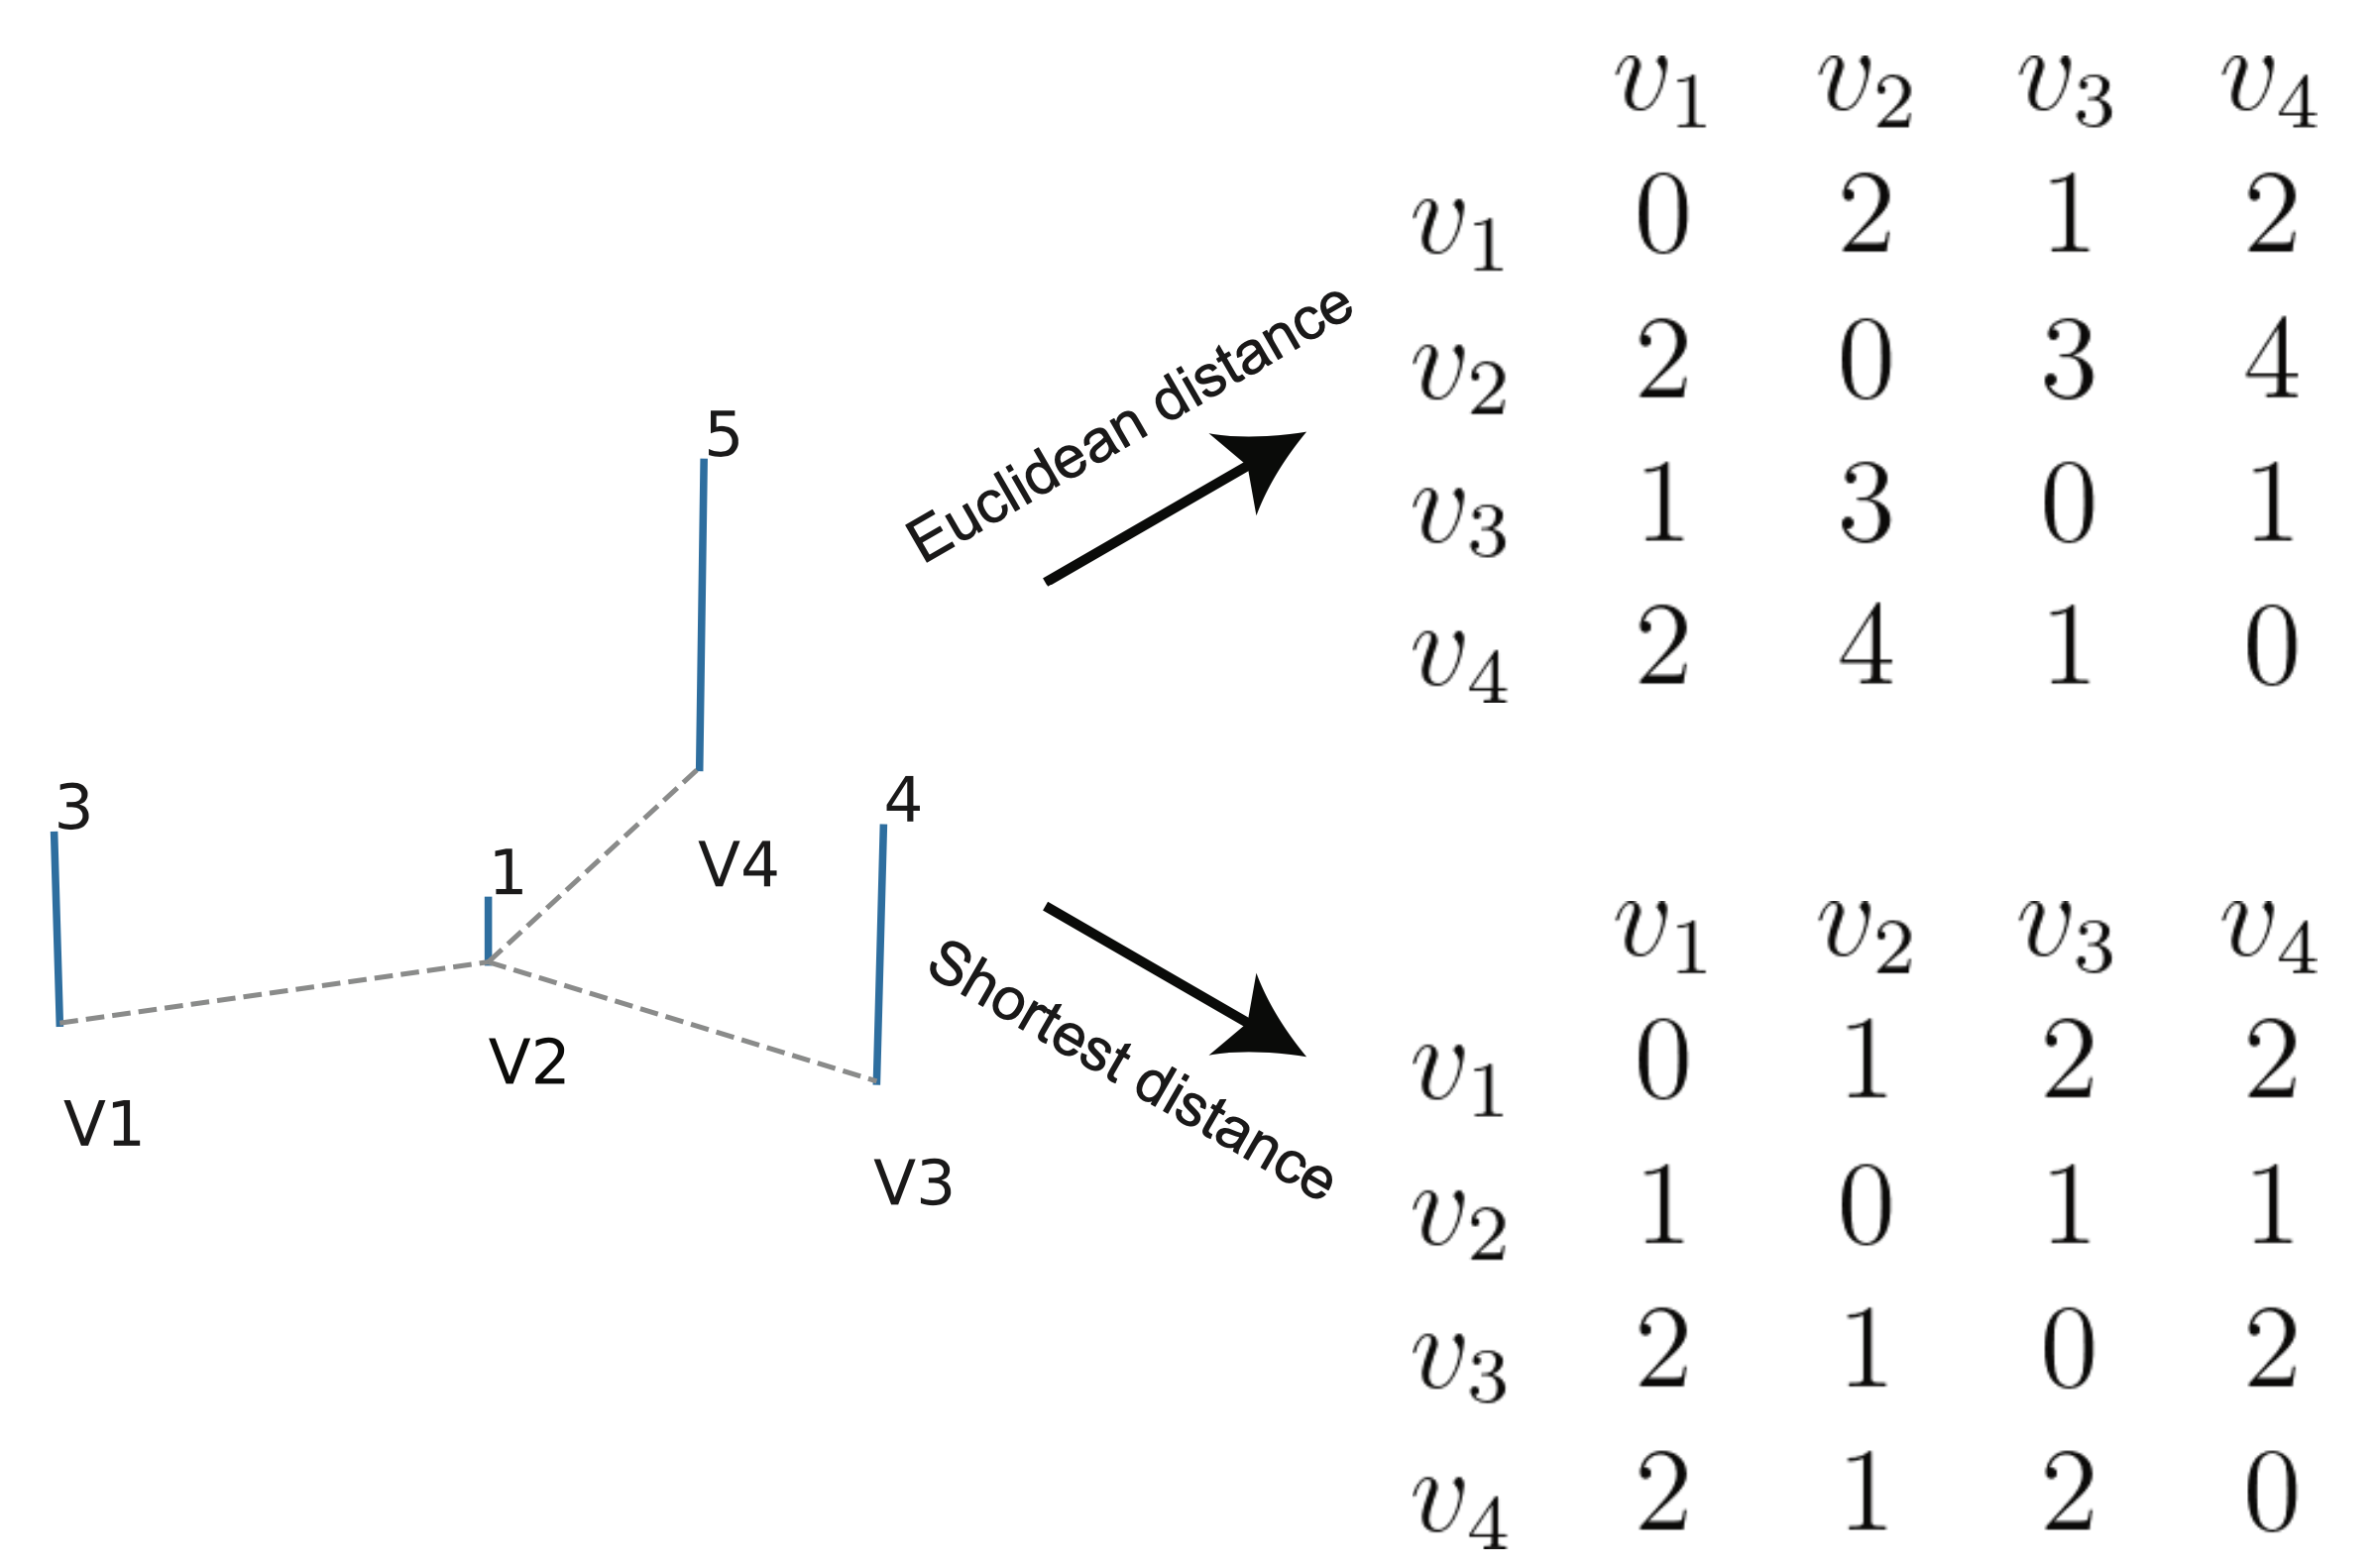
\includegraphics[width=0.8\textwidth,height=\textheight]{Beamer_files/figure-beamer/030e8263-46d1-4379-85b2-e3b509cc9119-1-39a1acd1-26dc-4cf6-91cd-fded8b949c72.png}

}

\caption{Fig6: The graph signal and its distance matrices}

\end{figure}%
\end{frame}

\begin{frame}{Proposed method (quick view)}
\phantomsection\label{proposed-method-quick-view-2}
Both two matrices look insufficient since they only use
\(({\cal V}, {\cal E})\) or \(f\).

\begin{itemize}
\tightlist
\item
  Euclidean distance matrix does not consider underlying structure
  \({\cal E}\).
\item
  Shortest distance matrix does not consider \(f\).
\end{itemize}

To consider both domain information, we propose the snow distance matrix
derived by the \textbf{\emph{heavysnow process}}.
\end{frame}

\begin{frame}{Proposed method (quick view)}
\phantomsection\label{proposed-method-quick-view-3}
\begin{block}{One realization of HS-process}
\begin{figure}[H]

{\centering 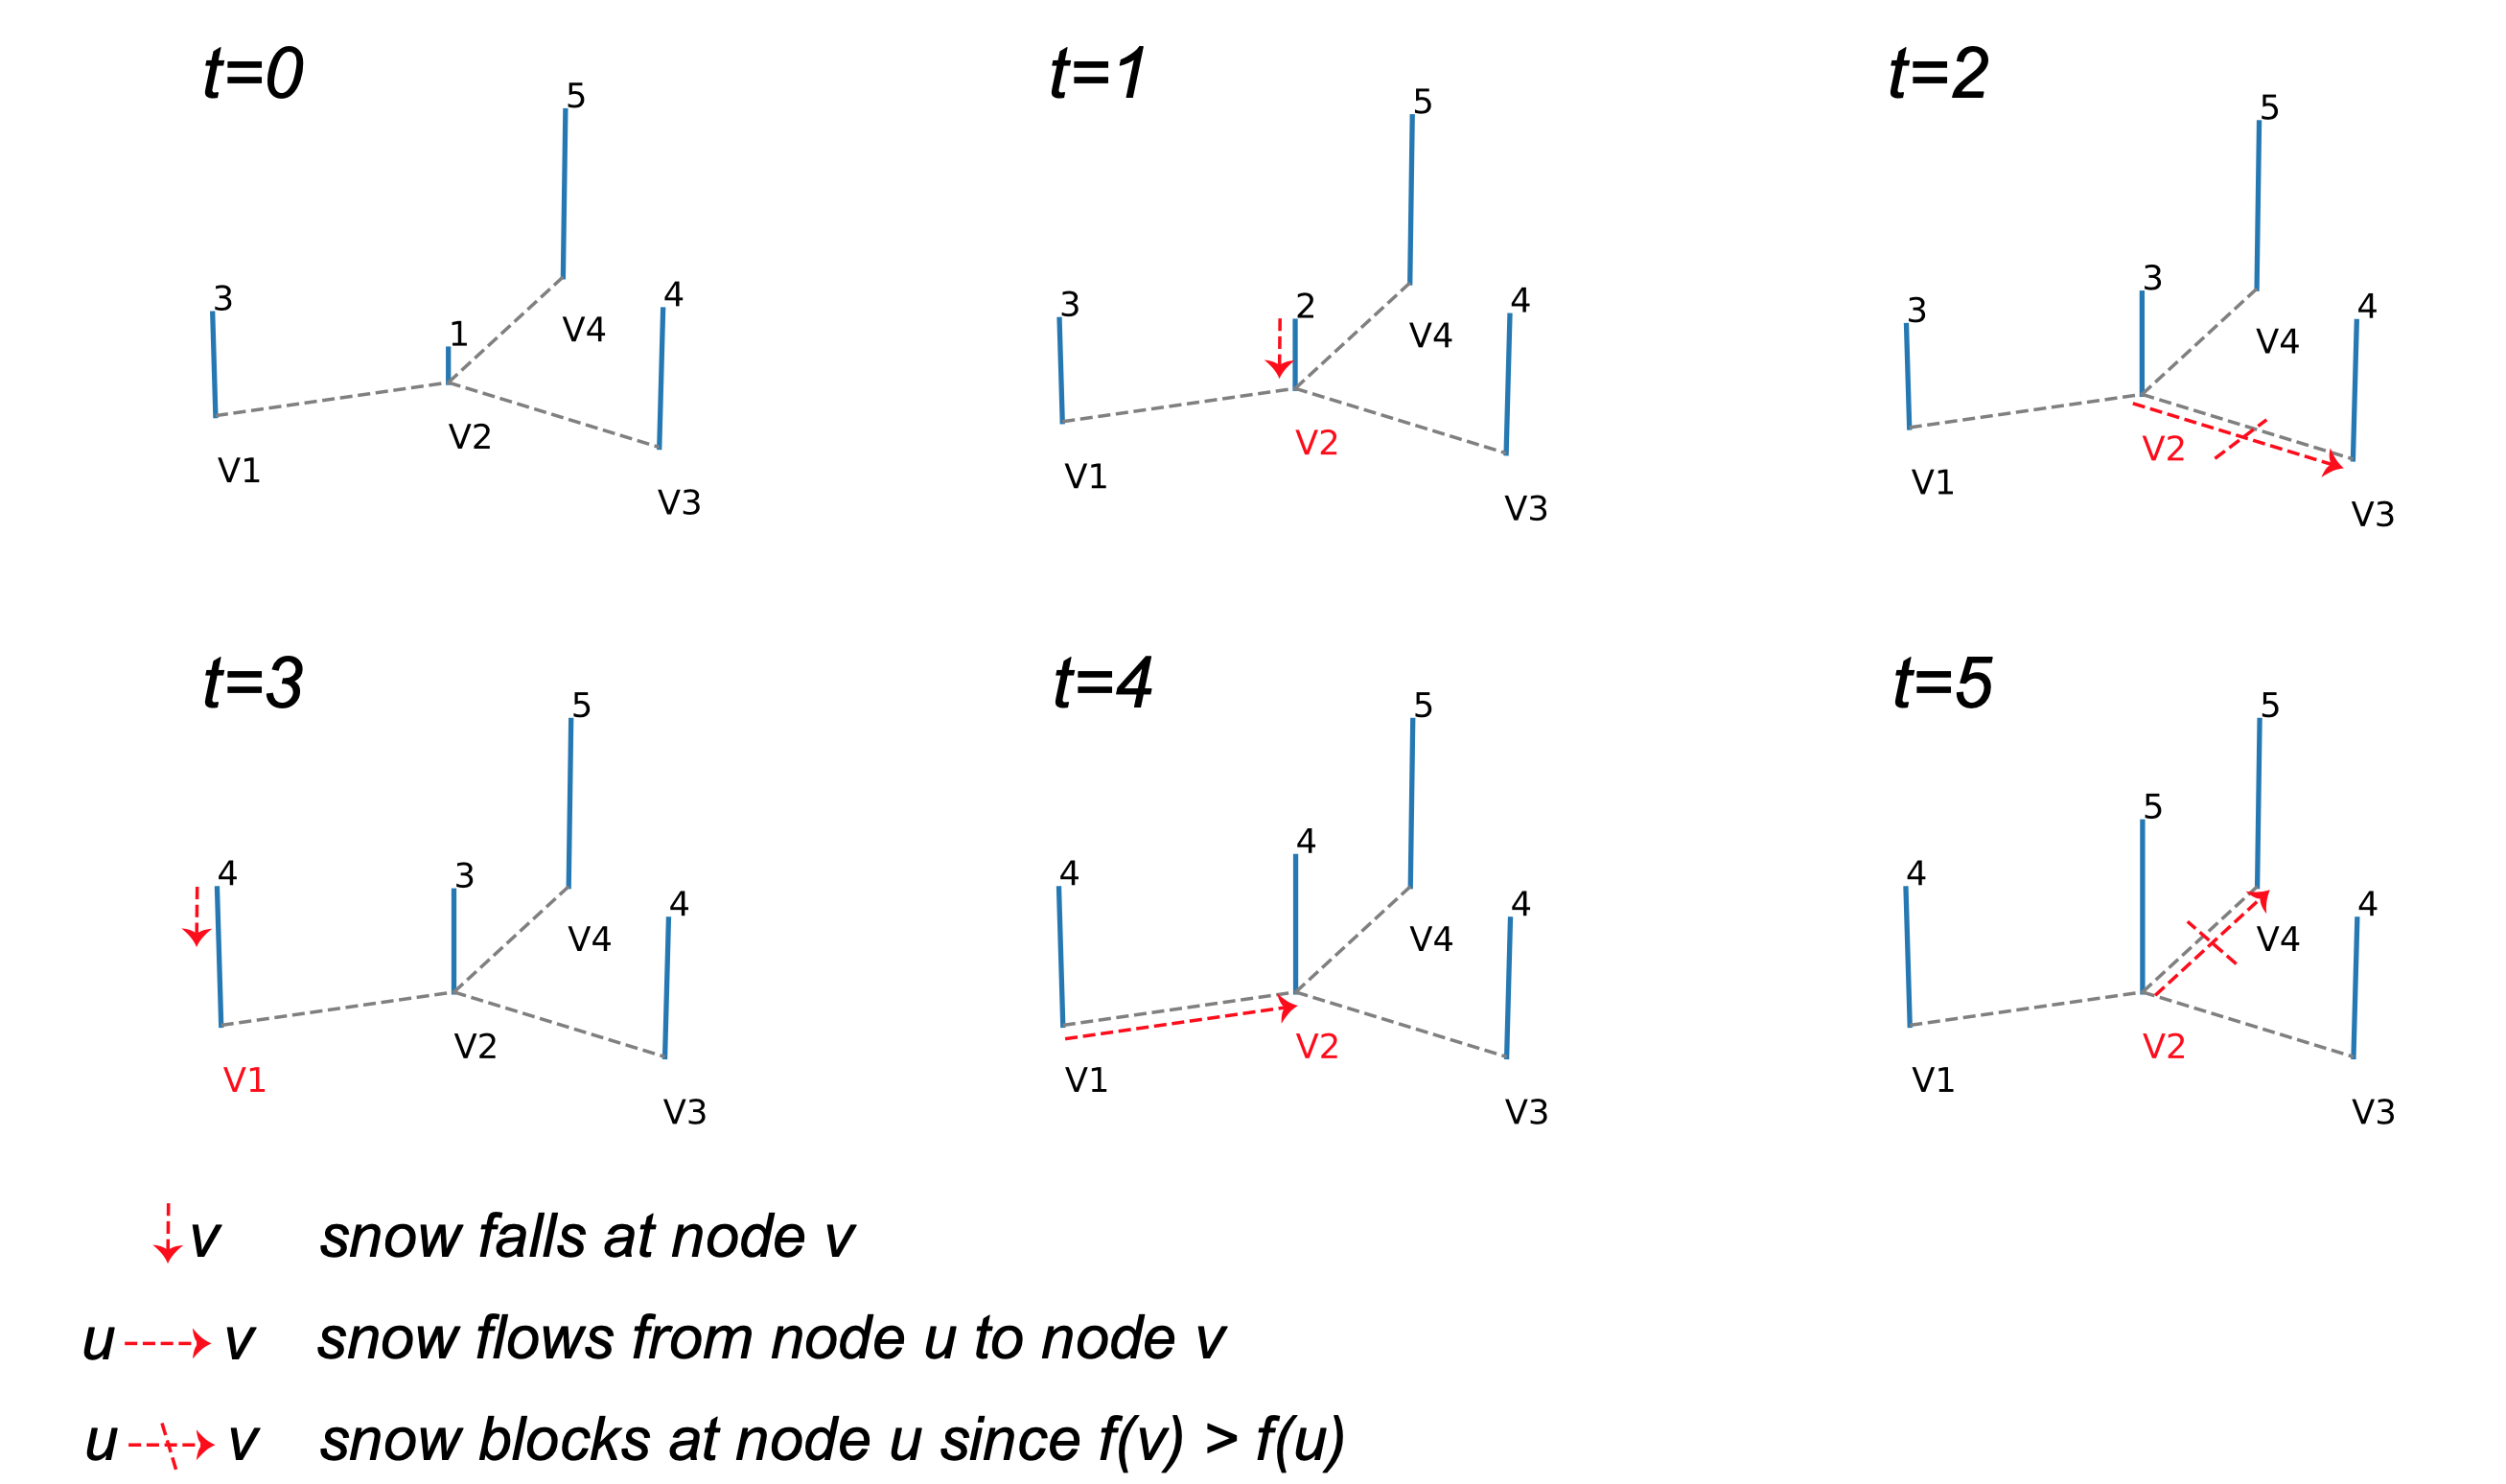
\includegraphics[width=0.6\textwidth,height=\textheight]{Beamer_files/figure-beamer/31efed2e-6ef1-4cf7-b2a6-d7bdbbcd7921-1-defed998-98ea-4c5a-ae0a-bd497d104889.png}

}

\caption{Fig7: Illustration of heavysnow process from \(t=0\) to
\(t=5\)}

\end{figure}%
\end{block}

\begin{block}{Snow distance}
\begin{itemize}
\tightlist
\item
  \(SD_{t=0}(v_1,v_2)=\|3-1\|_2\)
\item
  \(SD_{t=1}(v_1,v_2)=\|(3,3)-(1,2)\|_2\)
\item
  \(\dots\)
\item
  \(SD_{t=5}(v_1,v_2)=\|(3,3,3,4,4,4)-(1,2,3,3,4,5)\|_2\)
\end{itemize}
\end{block}
\end{frame}

\begin{frame}{Proposed method (quick view)}
\phantomsection\label{proposed-method-quick-view-4}
How to make snow distance small?

\begin{itemize}
\tightlist
\item
  To do this, \(v_1\) and \(v_2\) must have similar Euclidean values
\item
  and at the same time, \(v_1\) and \(v_2\) also be close in the network
  domain.
\end{itemize}

Note that

\begin{itemize}
\tightlist
\item
  Euclidean distance: only use \(f(v)\), \(v \in {\cal V}\).
\item
  Shortest distance: only use \(\{{\cal V}, {\cal E}\}\).
\item
  Snow distance: use \(\{{\cal V}, {\cal E}\}\) and \(f(v)\).
\end{itemize}
\end{frame}

\begin{frame}{Related studies}
\phantomsection\label{related-studies}
\begin{itemize}
\tightlist
\item
  Recently, non-Euclidean data is accumulating rapidly due to IT
  innovation. Thus analyzing non-Euclidean data is one of the most
  popular topics in recent years.
\item
  These research topics are collectively referred to as geometric deep
  learning (Bronstein et al. 2017; Cao et al. 2020), graph signal
  processing (Shuman et al. 2013), and graph learning (Xia et al. 2021).
\item
  There are two main approaches to analyze non-Euclidean data,
  \textbf{embedding technique} and \textbf{spectral analysis} (Cao et
  al. 2020).
\end{itemize}
\end{frame}

\begin{frame}{Related studies}
\phantomsection\label{related-studies-1}
\begin{block}{Embedding technique}
\phantomsection\label{embedding-technique}
\begin{itemize}
\tightlist
\item
  The embedding technique takes a two-step strategy to convert
  non-Euclidean data into Euclidean data and then apply existing
  statistical and machine learning methods.
\item
  This technique is also referred to as \textbf{manifold learning} or
  \textbf{nonlinear dimension reduction technique} (Bronstein et al.
  2017).
\end{itemize}
\end{block}
\end{frame}

\begin{frame}{Related studies}
\phantomsection\label{related-studies-2}
\begin{block}{Spectral analysis}
\phantomsection\label{spectral-analysis}
\begin{itemize}
\tightlist
\item
  Unlike the embedding technique, the spectral method uses the given
  data itself without transforming the non-Euclidean data into a
  Euclidean space.
\item
  Spectral methods necessarily include the common process of
  generalizing concepts such as \textbf{frequency} and
  \textbf{convolution} used in Euclidean space to non-Euclidean space.
\item
  This is done through calculating the eigenvector of the graph
  Laplacian, and then conducting the graph Fourier transform.
\end{itemize}
\end{block}
\end{frame}

\begin{frame}{Related studies}
\phantomsection\label{related-studies-3}
\textbf{Example of Spectral analysis}

\begin{block}{Spectral Clustering}
Spectral clustering is a technique for clustering non-Euclidean data
using the concept of \emph{smoothness} or \emph{bandwidth} of a graph
(Ng, Jordan, and Weiss 2001; Kipf and Welling 2016).
\end{block}

\begin{block}{GCN}
The graph convolutional neural network generalizes the convolution to
the non-Euclidean domain through the graph Fourier transform (Henaff,
Bruna, and LeCun 2015; Defferrard, Bresson, and Vandergheynst 2016;
Ktena et al. 2017).
\end{block}

\begin{block}{GSP}
Graph signal processing generalizes some concepts to non-Euclidean
domain via spectral domain:

\begin{figure}[H]

{\centering 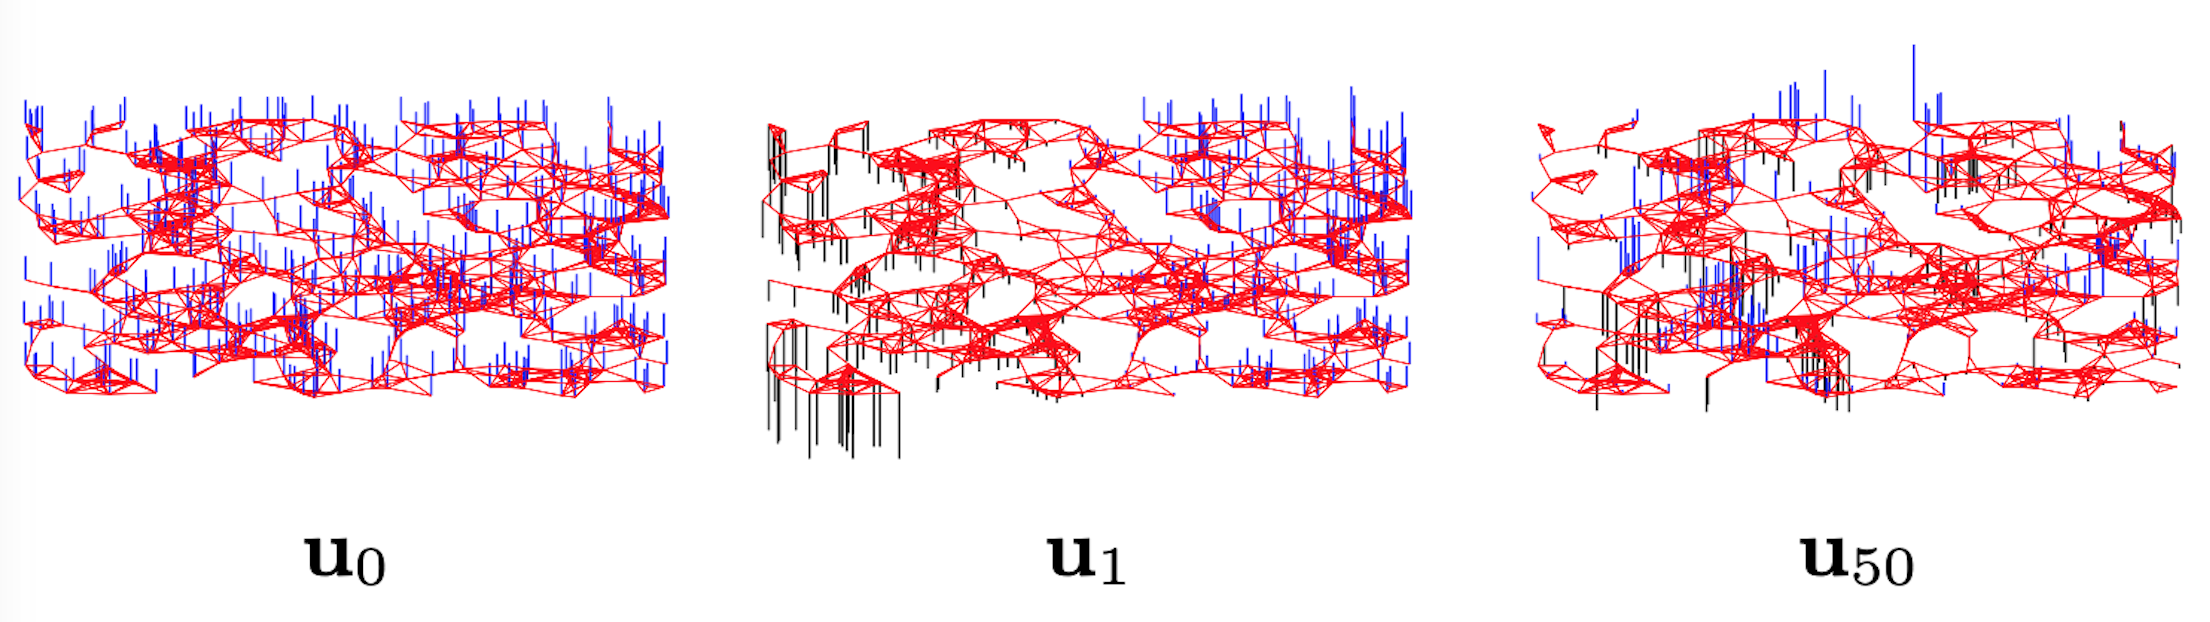
\includegraphics[width=0.6\textwidth,height=\textheight]{Beamer_files/figure-beamer/9796933e-0d46-4bf7-b743-4861031e15a2-1-639b753d-8966-45d6-a836-b805dbefc704.png}

}

\caption{Fig8: Three graph Laplacian eigenvectors of random sensor
network graph in Shuman et al. (2013).}

\end{figure}%
\end{block}
\end{frame}

\begin{frame}{Related studies}
\phantomsection\label{related-studies-4}
\textbf{Measure the similarity in non-Euclidean space}

Note that both embedding and spectral methods start with measuring the
distance or similarity between non-Euclidean data.

\begin{block}{Embedding}
To be specific, the embedding technique measures local affinity between
data, preserves it as much as possible, and embeds it into an
appropriate Euclidean space (Bronstein et al. 2017).
\end{block}

\begin{block}{Spectral}
The spectral method obtains an adjacency matrix or weighted adjacency
matrix of a graph signal, calculates the graph Laplacian, and interprets
eigenvalues and eigenvectors (Von Luxburg 2007).
\end{block}
\end{frame}

\begin{frame}{Related studies}
\phantomsection\label{related-studies-5}
A study on the similarity between non-Euclidean data is roughly divided
into a method that uses a random walk and a method that does not.

\begin{block}{Random walk based method}
\phantomsection\label{random-walk-based-method}
\begin{itemize}
\tightlist
\item
  Random walk means a random variable that moves randomly in given state
  space.
\item
  In the case of graph data, nodes can be interpreted as states.
\item
  Through the random walk, we can infer the underlying structure in the
  graph by examining nodes that are frequently met.
\end{itemize}
\end{block}
\end{frame}

\begin{frame}{Related studies}
\phantomsection\label{related-studies-6}
\textbf{Examples of random walk based method}

\begin{itemize}
\tightlist
\item
  Diffusion distance (\textbf{coifman2006diffusion?})
\item
  Euclidean commute time distance (\textbf{yen2005clustering?};
  \textbf{saerens2004principal?})
\item
  In addition, there are many studies that infer the intrinsic structure
  of non-Euclidean data based on random walks
  (\textbf{perozzi2014deepwalk?}; \textbf{grover2016node2vec?}).
\end{itemize}
\end{frame}

\begin{frame}{Related studies}
\phantomsection\label{related-studies-7}
\begin{itemize}
\tightlist
\item
  Heat diffusion on non-Euclidean domains
\end{itemize}

\begin{figure}[H]

{\centering 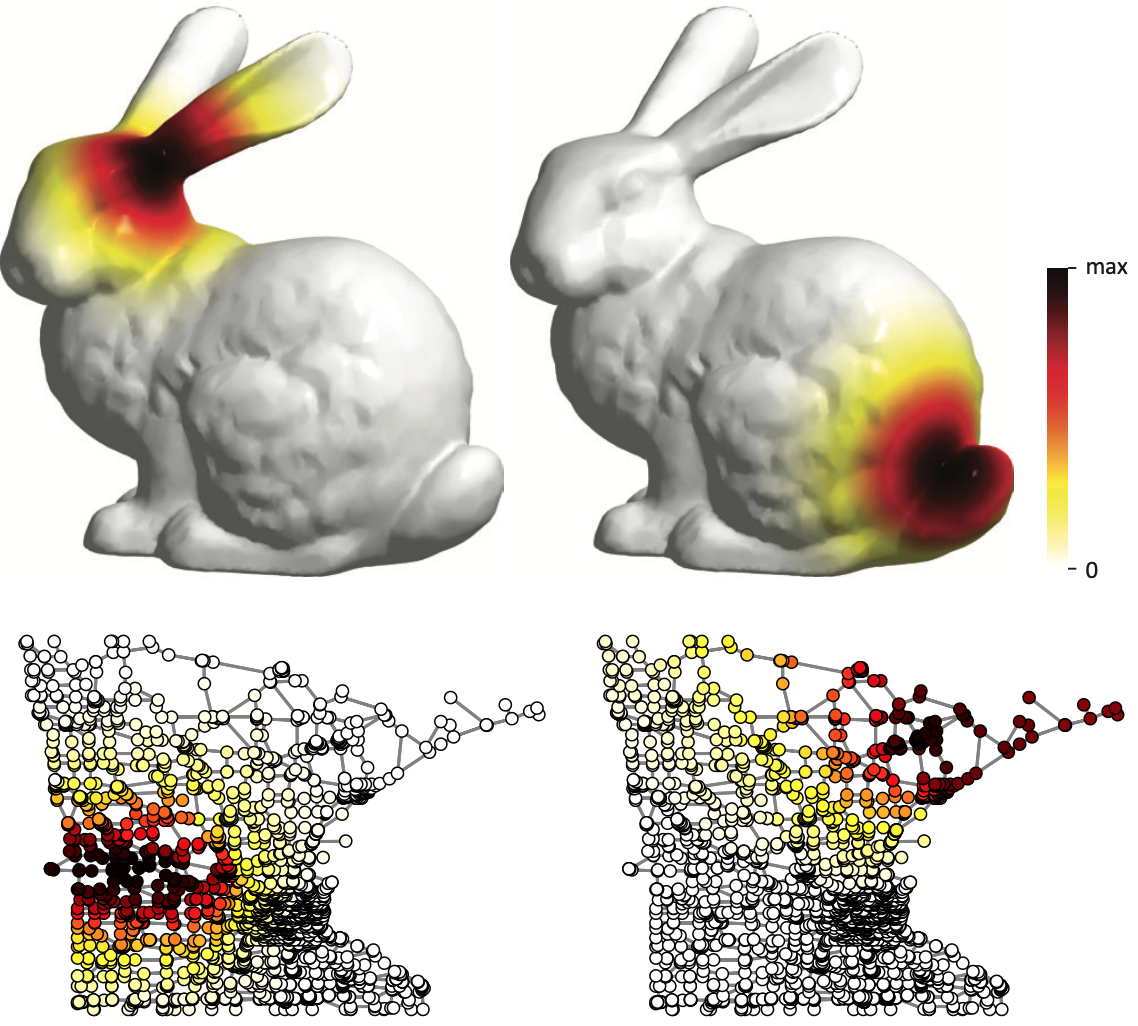
\includegraphics{Beamer_files/figure-beamer/ac3d5964-07e8-4bac-9d27-53a787729469-1-ddbd0c7d-ac06-4c45-bcda-1eecbd716cd3.png}

}

\caption{Fig9: Examples of heat kernels on non-Euclidean domains
(manifold, top; and graph, bottom) from Bronstein et al. (2017)}

\end{figure}%
\end{frame}

\begin{frame}{Related studies}
\phantomsection\label{related-studies-8}
\begin{block}{Other method}
\phantomsection\label{other-method}
\begin{itemize}
\tightlist
\item
  There are also methods that infer an intrinsic structure without being
  based on a random walk.
\item
  Examples are the shortest distance and the resistance distance
  (\textbf{klein1993resistance?})
\end{itemize}
\end{block}
\end{frame}

\begin{frame}{Proposed method}
\phantomsection\label{proposed-method}
\textbf{Stage 1}

\begin{itemize}
\tightlist
\item
  Define the heavysnow process, snow-distance matrix.
\item
  Proof some properties in heavysnow process.
\end{itemize}

\textbf{Stage 2}

\begin{itemize}
\tightlist
\item
  Embedding technique with snow-distance matrix.
\item
  Spectral analysis with snow-weight matrix. (Note that it derive the
  new graph Laplacian.)
\end{itemize}
\end{frame}

\begin{frame}{Proposed method}
\phantomsection\label{proposed-method-1}
\textbf{Some challenges}

\begin{itemize}
\tightlist
\item
  Can we prove the weak ergodicity of the heavysnow process?
\item
  Is the snow distance better than the weighted sum of diffusion
  distance and Euclidean distance?
\item
  Can we reduce the wiggly effect\footnote<.->{which occurs due to the
    non-homogeneos markov chain}?
\item
  Can we reduce the computational time?
\end{itemize}
\end{frame}

\begin{frame}{Proposed method}
\phantomsection\label{proposed-method-2}
\begin{block}{Topic 1: Weak ergodicity}
\phantomsection\label{topic-1-weak-ergodicity}
\begin{block}{Thoerem 1}
\phantomsection\label{thoerem-1}
Let \({\cal G}=(V,{\bf E},{\bf W})\) be a weighted graph with \(|V|=n\)
and \({\bf f}\) be a graph signal defined on \({\cal G}\),
\({\cal H}(t)\) denote the heavy-snow transformation of
\((f,{\cal G})\), and \(\{X_t\}\) as trace of snow. Then, \(\{X_t\}\) is
ergodic in the weak sense.
\end{block}

\begin{block}{Our strategies}
\phantomsection\label{our-strategies}
\begin{itemize}
\tightlist
\item
  Assume finite state space, i.e., assume \(|V|=n <\infty\).
\item
  Set \(T_{max} < \infty\) where \(T_{max}\) means the maximum number of
  times that can flow.
\end{itemize}
\end{block}
\end{block}
\end{frame}

\begin{frame}{Proposed method}
\phantomsection\label{proposed-method-3}
\begin{block}{Topic 2: Distance}
\phantomsection\label{topic-2-distance}
\begin{figure}[H]

{\centering 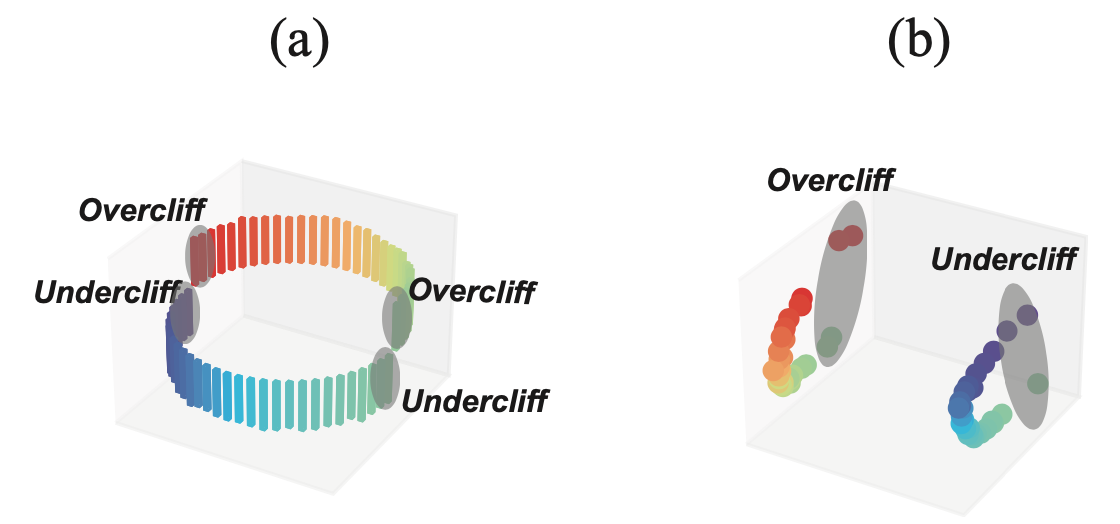
\includegraphics{Beamer_files/figure-beamer/2e91521c-95a3-433e-9db0-ef5600641715-1-1bd48489-4286-427e-a563-867c2d28f871.png}

}

\caption{Fig10: (a) Manifold valued data. (b) Embedding result produced
by snow distance matrix.}

\end{figure}%
\end{block}
\end{frame}

\begin{frame}{Proposed method}
\phantomsection\label{proposed-method-4}
\begin{block}{Topic 3: Embedding}
\phantomsection\label{topic-3-embedding}
\begin{figure}[H]

{\centering 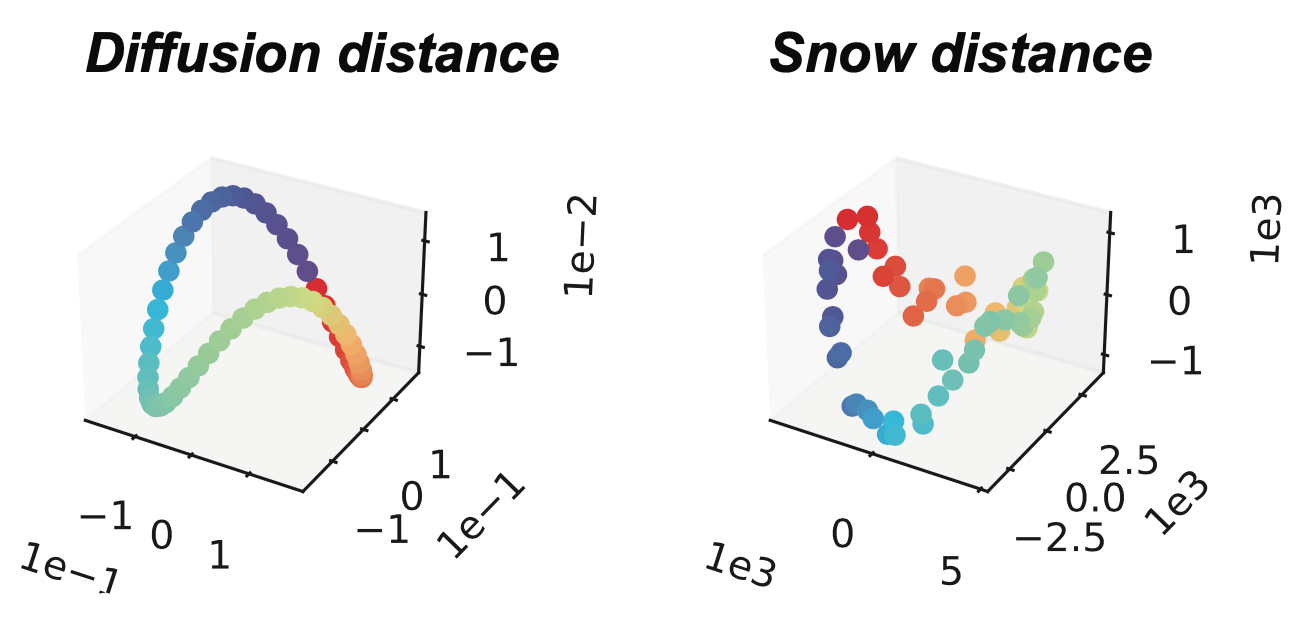
\includegraphics{Beamer_files/figure-beamer/8683c9db-2fa6-49e6-95a4-7597b31595ca-1-157cf8b1-35f3-4a36-9141-b40be68b343a.png}

}

\caption{Fig11: Embedding results from diffusion distance (left) and
snow distance (right)}

\end{figure}%

\begin{block}{Our strategies}
\phantomsection\label{our-strategies-1}
\begin{itemize}
\tightlist
\item
  Compute multiple processes and average that.
\item
  Reduce the amount of falling snow and increase \(t\).
\end{itemize}
\end{block}
\end{block}
\end{frame}

\begin{frame}{Proposed method}
\phantomsection\label{proposed-method-5}
\begin{block}{Topic 4: Decomposition}
\phantomsection\label{topic-4-decomposition}
\end{block}

\begin{block}{Data}
\begin{figure}[H]

{\centering 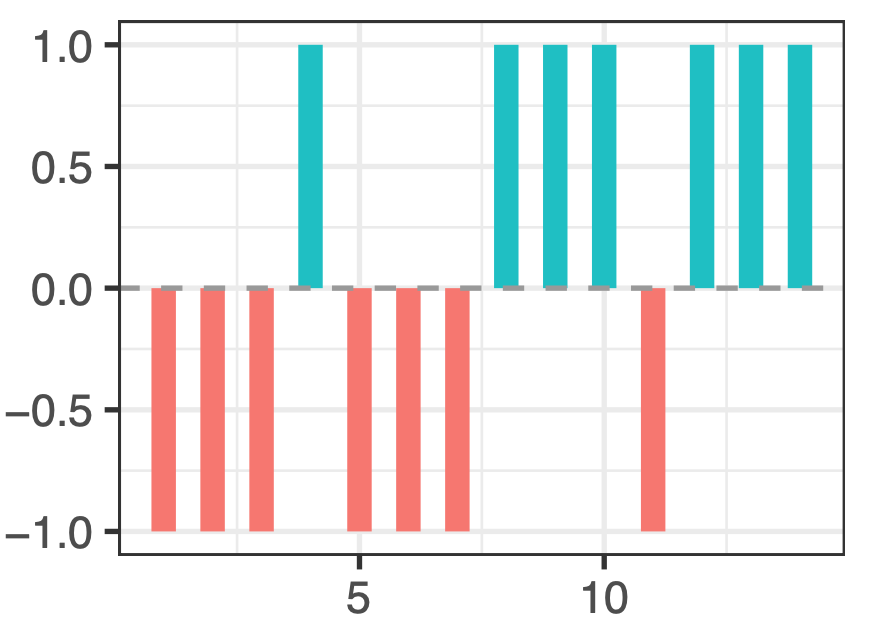
\includegraphics[width=0.4\textwidth,height=\textheight]{Beamer_files/figure-beamer/1330f074-21c6-48a3-b7bb-56b2c6aa30df-1-0a985073-2a42-4c15-b4ee-e1f0b426939b.png}

}

\caption{Fig12: Simple graph signal with 14 nodes.}

\end{figure}%
\end{block}

\begin{block}{GSO}
Define the normal graph shift operator as

\[{\bf S} = 
\begin{bmatrix} 
0 &1 &0 &\dots & 0 \\ 
0 &0 &1 &\dots & 0 \\ 
\dots & \dots & \dots &\dots & \dots \\ 
0 &0 &0 &\dots & 1 \\ 
1 &0 &0 &\dots & 0
\end{bmatrix}.\]
\end{block}

\begin{block}{HST}
Apply HST with \({\bf S}\) and get the snow graph Laplacian
\({\bf L}_{snow}\).
\end{block}

\begin{block}{Eigen}
\begin{figure}[H]

{\centering 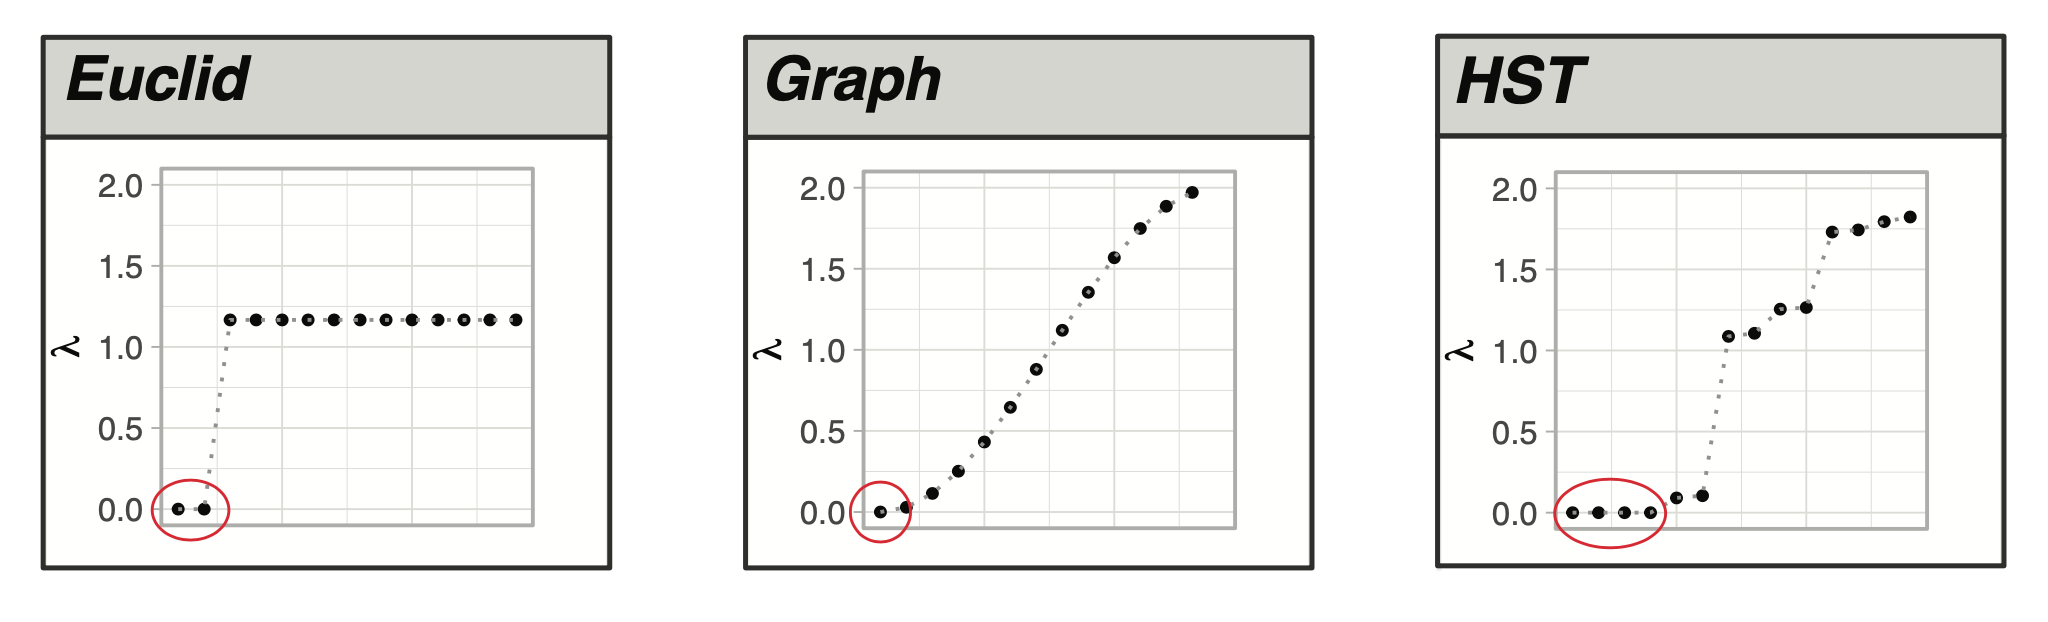
\includegraphics{Beamer_files/figure-beamer/1330f074-21c6-48a3-b7bb-56b2c6aa30df-3-709737c2-a885-44b6-97ad-74872801614e.png}

}

\caption{Fig13: Eigenvalues obtained by three graph Laplacians}

\end{figure}%
\end{block}

\begin{block}{Decomp1}
\begin{figure}[H]

{\centering 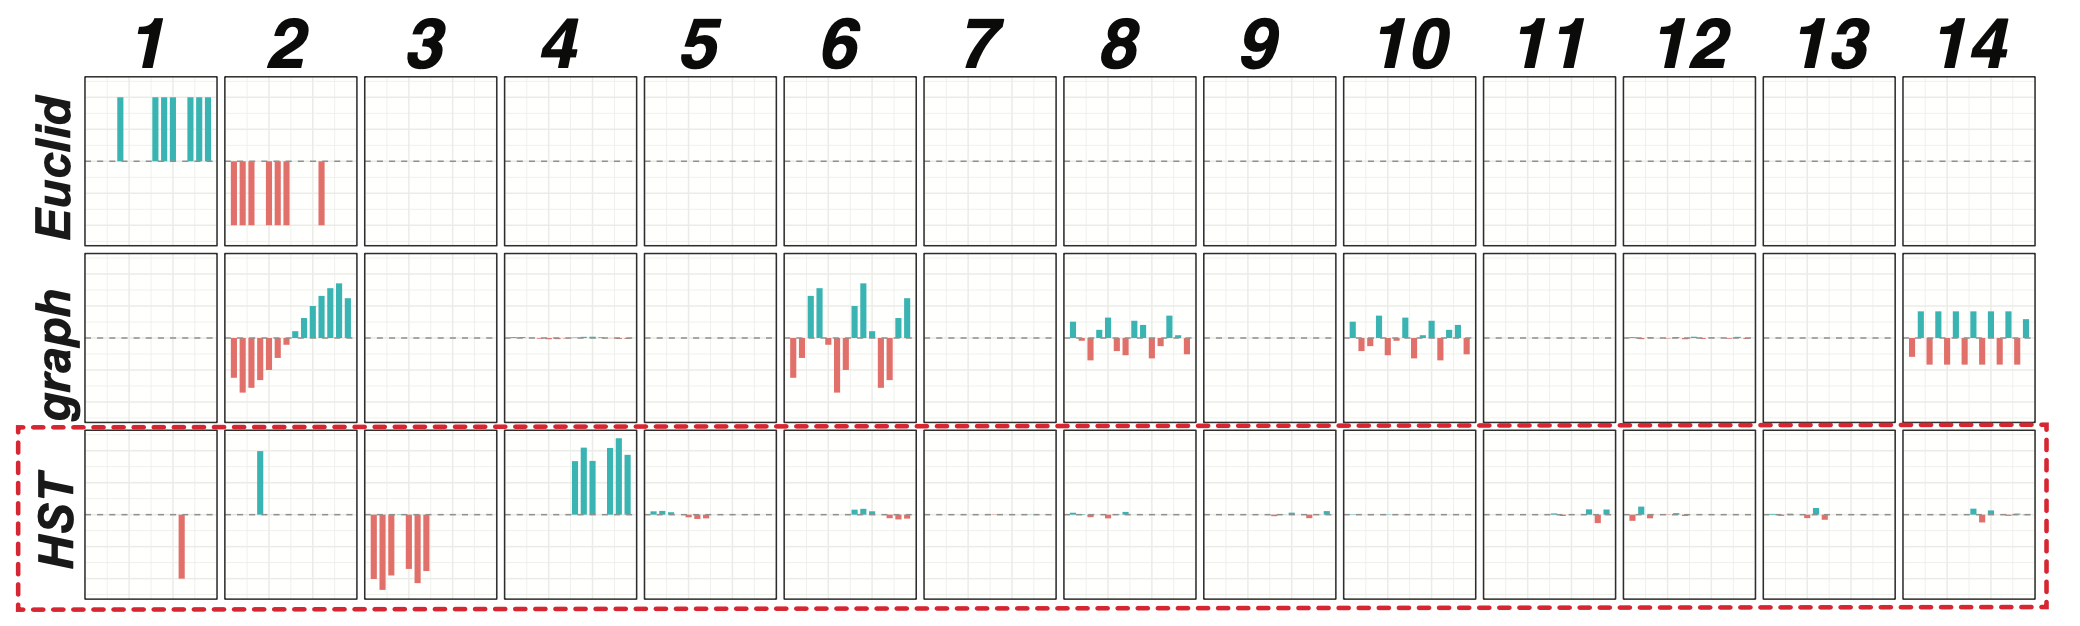
\includegraphics{Beamer_files/figure-beamer/1330f074-21c6-48a3-b7bb-56b2c6aa30df-2-22f5c831-a35f-455d-9060-a267cff75f6c.png}

}

\caption{Fig14: The decomposition results by three graph Laplacians.}

\end{figure}%
\end{block}

\begin{block}{Decomp2}
\begin{figure}[H]

{\centering 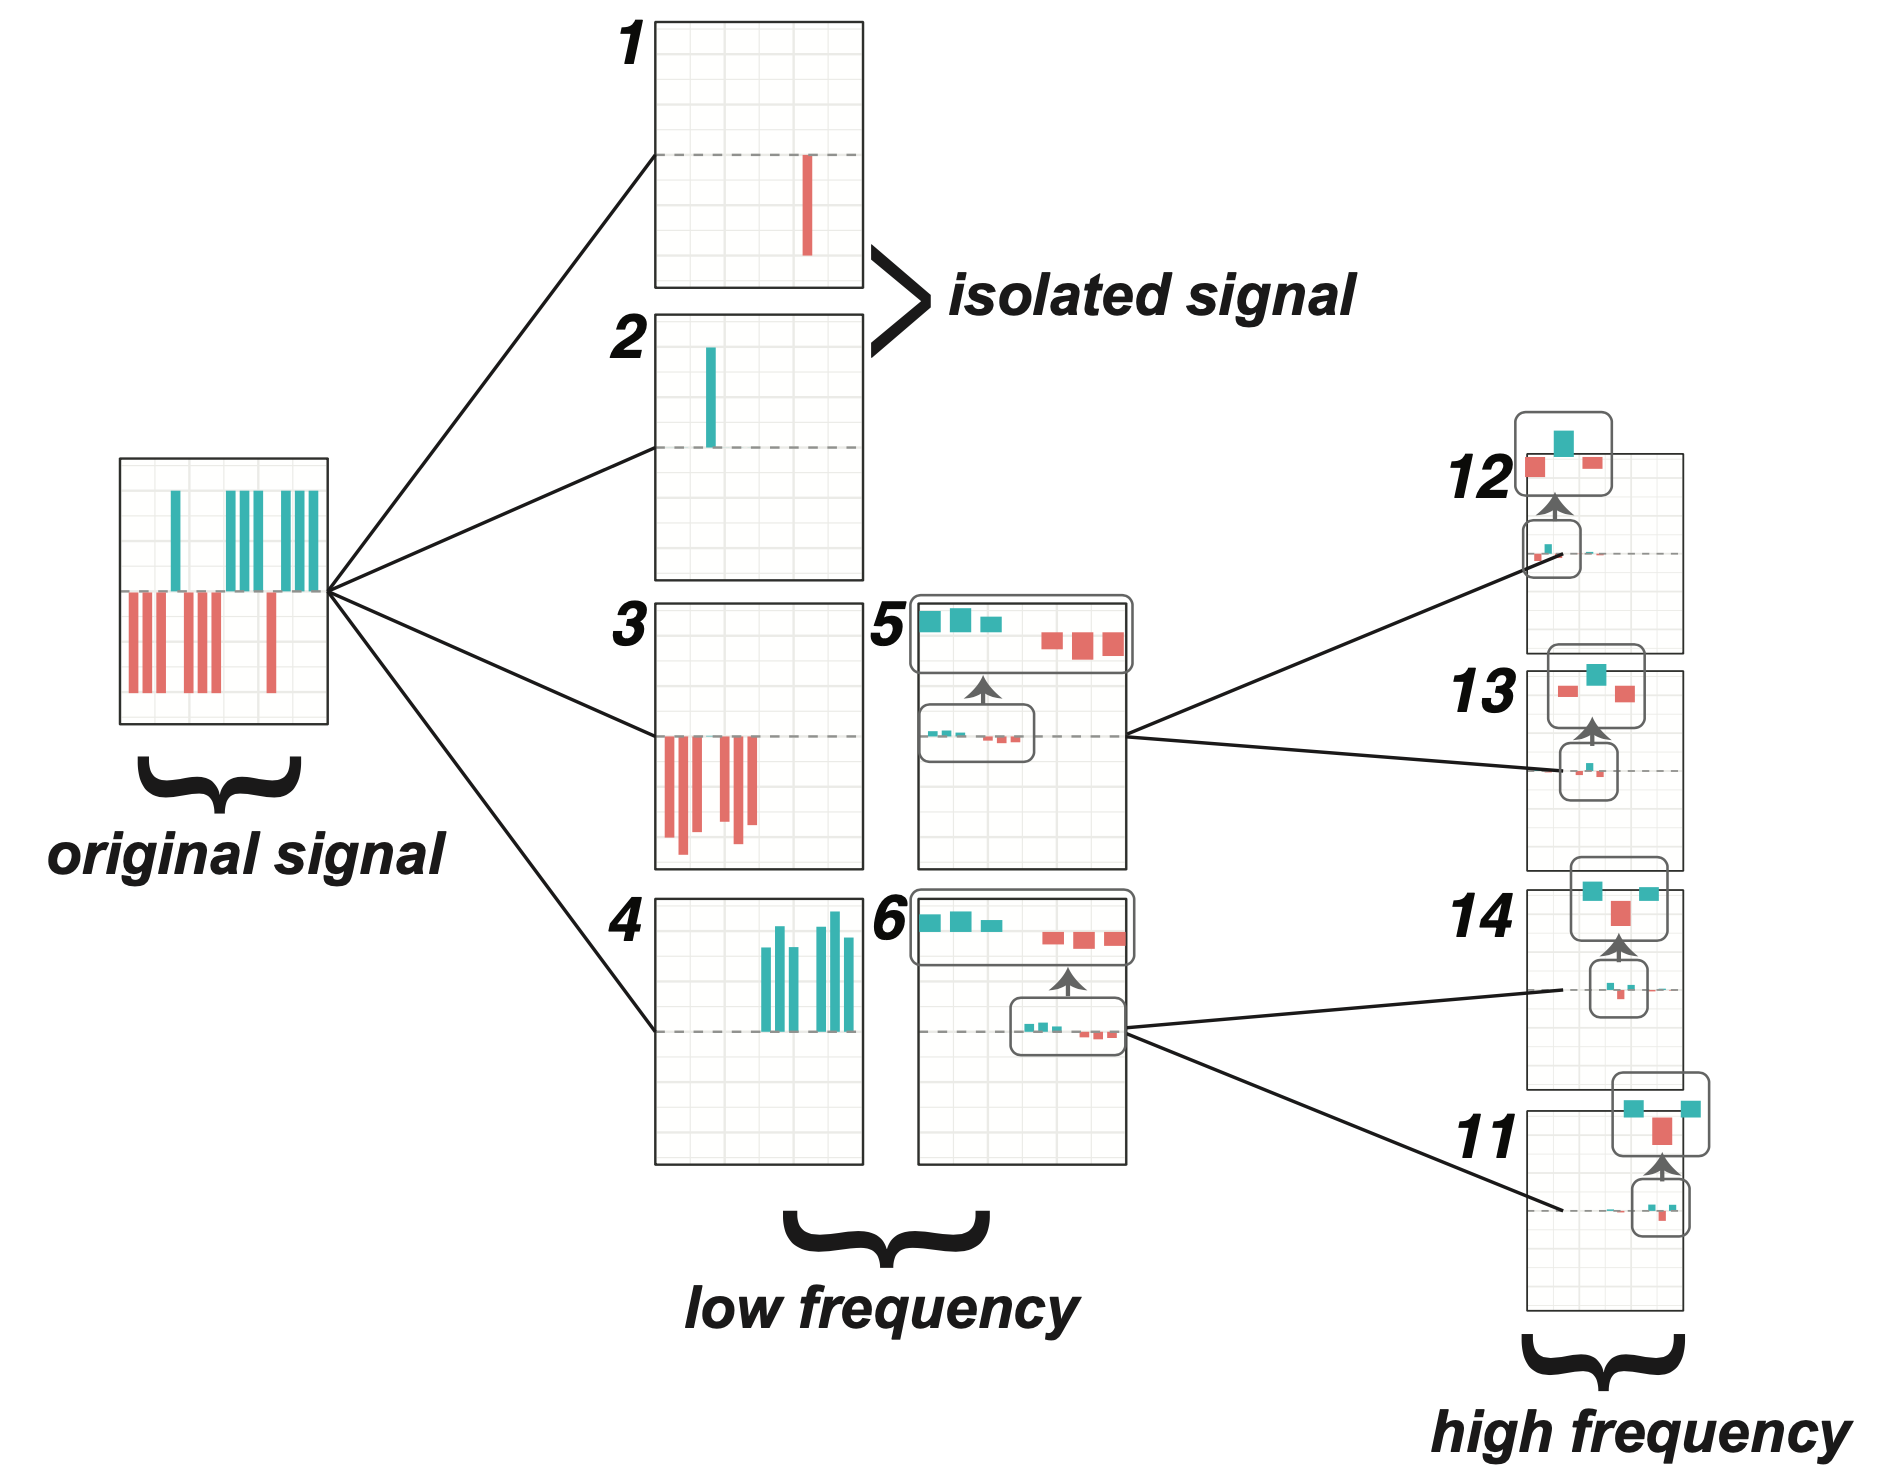
\includegraphics[width=0.5\textwidth,height=\textheight]{Beamer_files/figure-beamer/1330f074-21c6-48a3-b7bb-56b2c6aa30df-4-ef4af1fd-a8b8-4cda-b186-aa1d9f14c775.png}

}

\caption{Fig15: An enlarged illustration of the components by the snow
graph Laplacian.}

\end{figure}%
\end{block}
\end{frame}

\begin{frame}{Proposed method}
\phantomsection\label{proposed-method-6}
\begin{block}{Topic 5: Calculation time}
\phantomsection\label{topic-5-calculation-time}
\begin{block}{Our strategies}
\phantomsection\label{our-strategies-2}
\begin{itemize}
\tightlist
\item
  Compute multiple processes in parallel.
\item
  Drop snow on multiple nodes at the same time.
\end{itemize}
\end{block}
\end{block}
\end{frame}

\begin{frame}{Real data analysis}
\phantomsection\label{real-data-analysis}
\textbf{\emph{Marvel Cinematic Universe (MCU)}}

\begin{itemize}
\tightlist
\item
  For analysis, we use 23 superhero movies released by Marvel Studios
  since 2008.
\item
  \textbf{Networks}: These films are in the MCU, a shared universe
  created by Marvel Studios. So, each movie shares characters, settings,
  plots, and stories with other movies from the MCU. Therefore, it can
  be considered that a certain network exists between the films.
\item
  \textbf{Euclidean value}: Each movie has a different box-office
  record, which can be interpreted as a Euclidean signal defined on the
  network domain.
\end{itemize}
\end{frame}

\begin{frame}{Real data analysis}
\phantomsection\label{real-data-analysis-1}
\textbf{Problem Settings}

\begin{block}{Euclidean value}
\begin{itemize}
\tightlist
\item
  \({\cal V}:=\) set of films
\item
  \({\bf f}:=\) box-office record of each film
\end{itemize}
\end{block}

\begin{block}{Networks}
\begin{itemize}
\item
  \({\bf W}:=\) strength of connection between films
\item
  To obtain the elements of \(\bf W\), we examine all the characters in
  each movie and measure how many characters overlap between them.
\item
  All information about characters is obtained from
  \url{https://www.imdb.com/list/ls031310794/}, a database related to
  films.
\end{itemize}
\end{block}
\end{frame}

\begin{frame}{Real data analysis}
\phantomsection\label{real-data-analysis-2}
\begin{figure}[H]

{\centering 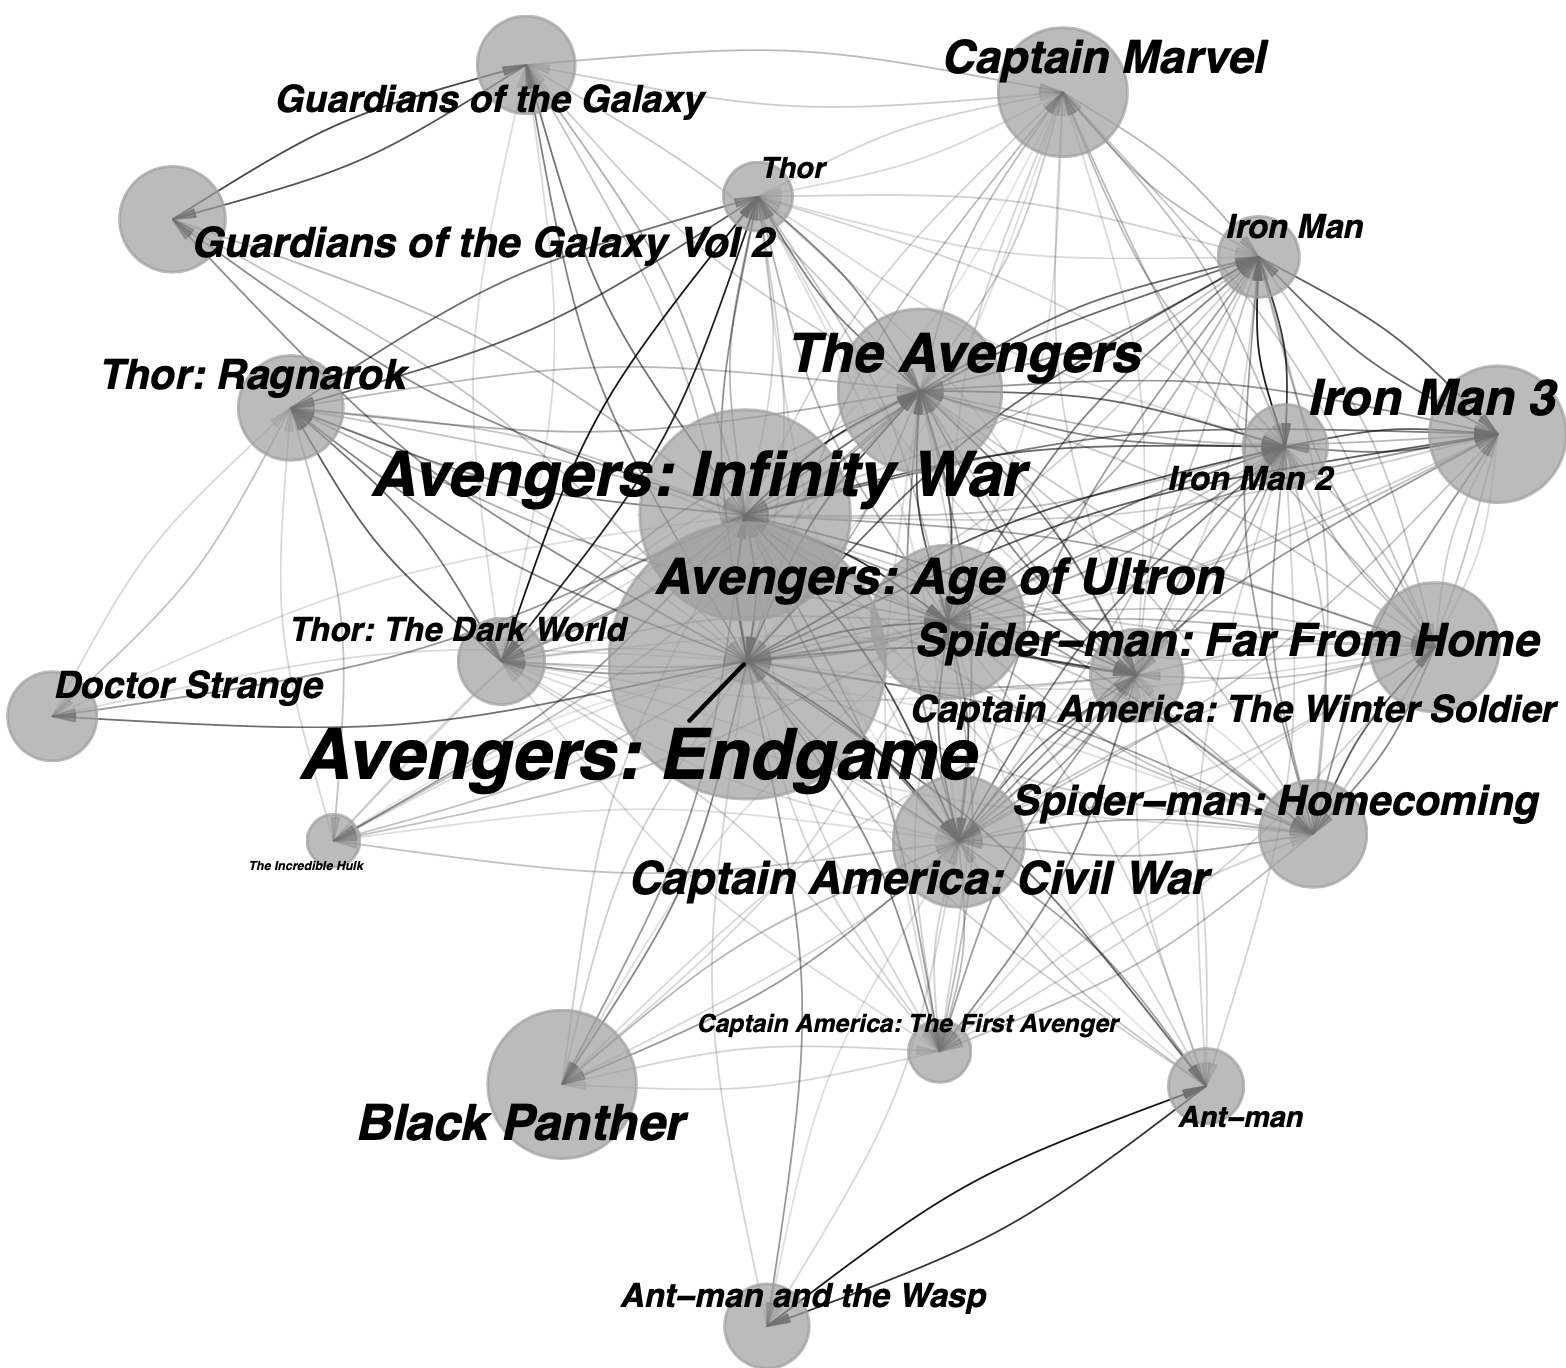
\includegraphics{Beamer_files/figure-beamer/731cd6ca-1909-4d11-abaf-7c54dc27a171-1-960ea596-34b9-4342-9092-3f9ceb658db7.png}

}

\caption{Fig16: Graph signal \(f\) on MCU networks
\(({\cal V},{\bf W})\); The value of \(f\) represented in size of vertex
and weight of nodes represented by with of line.}

\end{figure}%
\end{frame}

\begin{frame}{Real data analysis}
\phantomsection\label{real-data-analysis-3}
Movies can be classified according to the response to the question:

\begin{enumerate}
\tightlist
\item
  Was it a successful film?
\item
  Will there be heroes who play a central role?
\item
  Are there multi-heroes?
\end{enumerate}
\end{frame}

\begin{frame}{Real data analysis}
\phantomsection\label{real-data-analysis-4}
\begin{enumerate}
\tightlist
\item
  A \emph{successful film} is one that attracts a large audience.
\item
  The \emph{main hero} is defined as a hero who is influential enough to
  appear frequently in other solo hero movies. Iron Man, Captain
  America, and Thor are the main heroes.
\item
  The \emph{multi-hero movies} include Avengers 1-4 and Captain America:
  Civil War. In these films, many heroes unite to fight a powerful
  enemy, or heroes confront each other because of ideological
  differences.
\end{enumerate}
\end{frame}

\begin{frame}{Real data analysis}
\phantomsection\label{real-data-analysis-5}
\begin{figure}[H]

{\centering 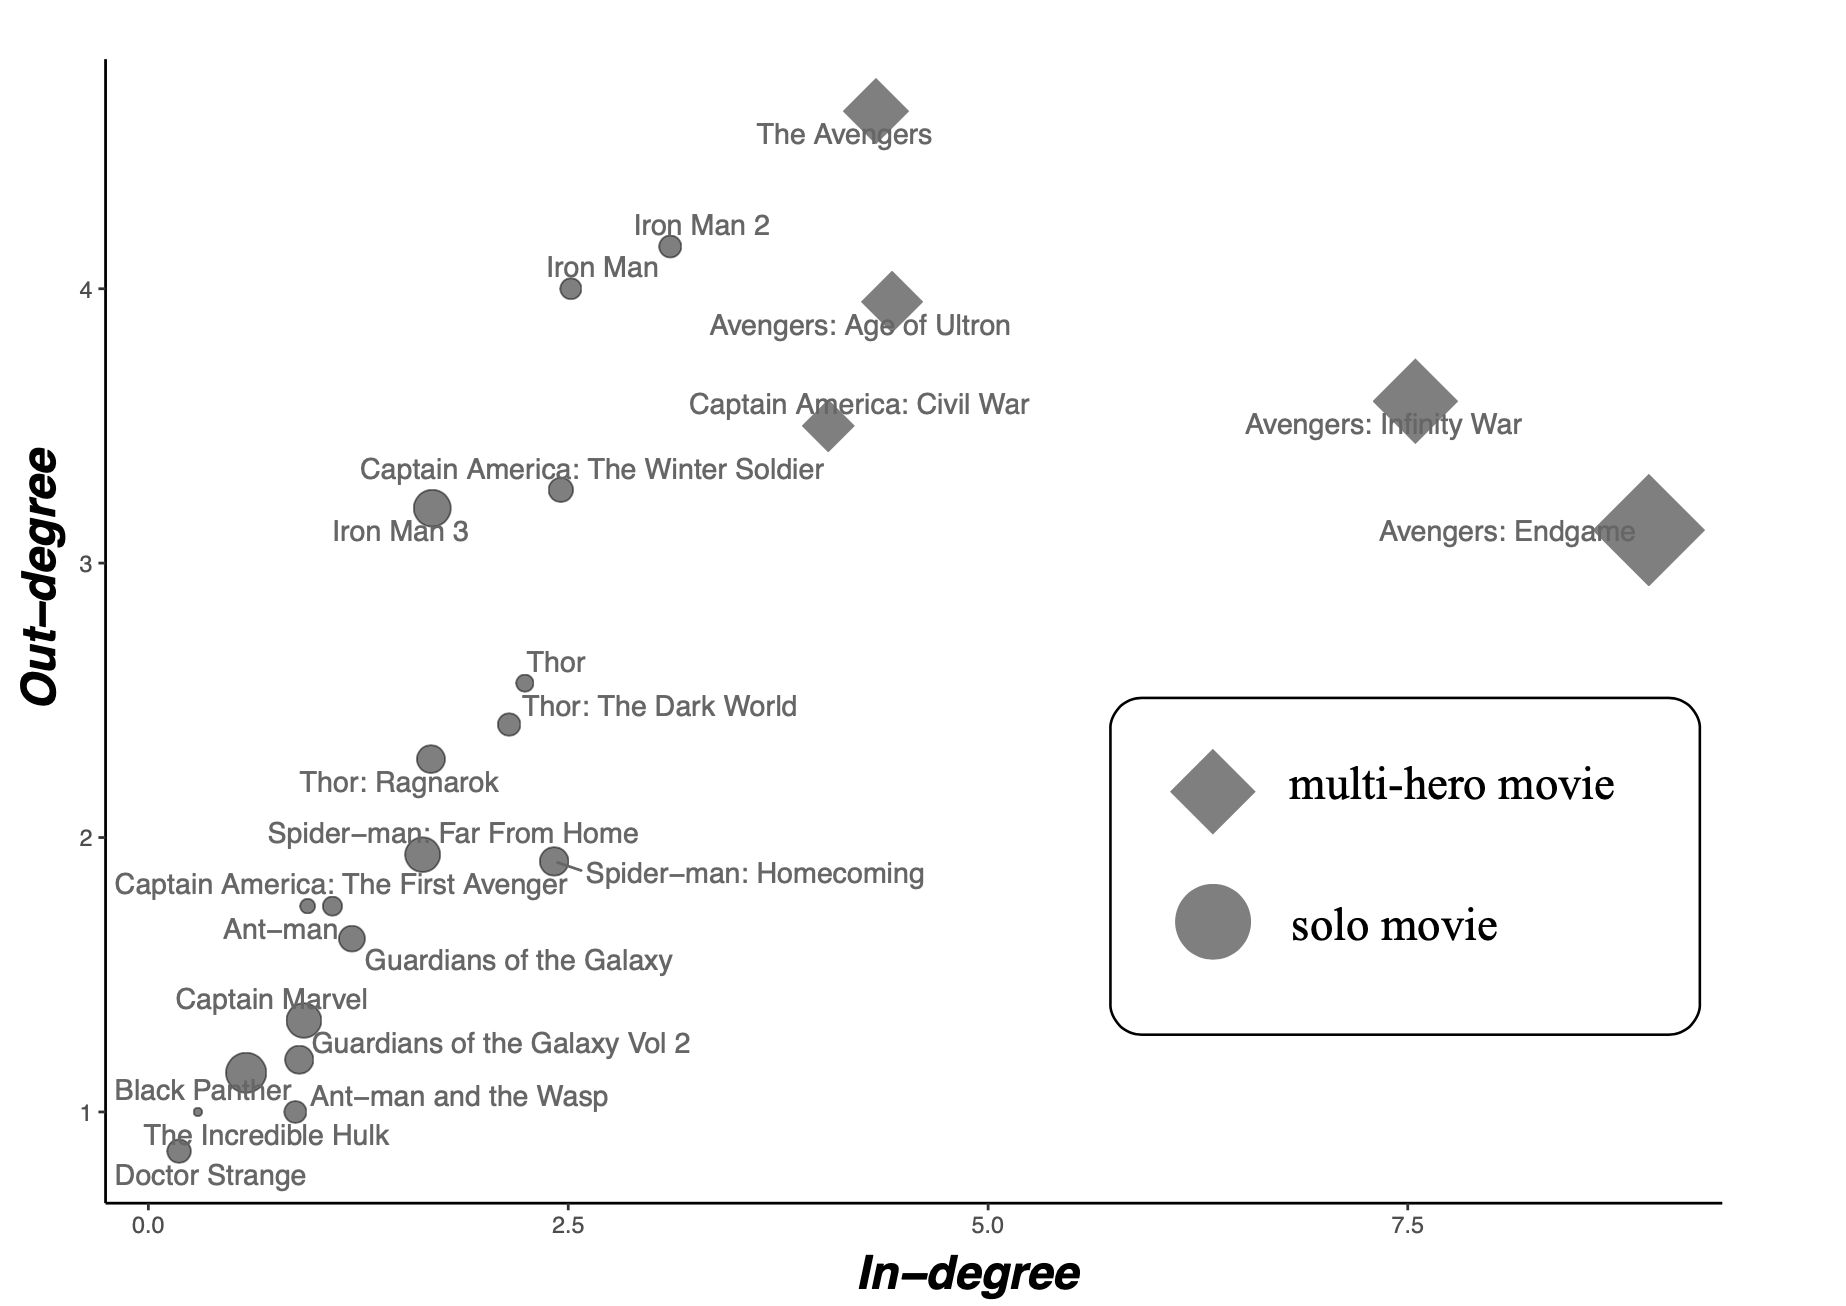
\includegraphics{Beamer_files/figure-beamer/8999da2d-1900-4008-bf11-3c8d4936bf52-1-16d3a795-5a96-46a9-b379-52f4daad4ccb.png}

}

\caption{Fig17: Visulization of MCU data}

\end{figure}%
\end{frame}

\begin{frame}{Real data analysis}
\phantomsection\label{real-data-analysis-6}
\begin{block}{1}
\begin{figure}[H]

{\centering \includegraphics{MCU_decomp1.png}

}

\caption{Fig18: comp1-- mean(?) of MCU data}

\end{figure}%
\end{block}

\begin{block}{2}
\begin{figure}[H]

{\centering \includegraphics{MCU_decomp2.png}

}

\caption{Fig19: comp2-- low frequency of MCU data; (red) main hero
(blue) minor hero}

\end{figure}%
\end{block}

\begin{block}{5}
\begin{figure}[H]

{\centering \includegraphics{MCU_decomp3.png}

}

\caption{Fig20: comp5-- sub-wave of main hero; (red) movies with one
main hero (blue) multi-hero movies}

\end{figure}%
\end{block}

\begin{block}{17}
\begin{figure}[H]

{\centering \includegraphics{MCU_decomp4.png}

}

\caption{Fig20: comp17-- sub-wave of minor hero; (red) less successful
films with minor heroes (blue) successful films with minor heroes}

\end{figure}%
\end{block}

\begin{block}{19}
\begin{figure}[H]

{\centering \includegraphics{MCU_decomp5.png}

}

\caption{Fig21: comp19-- two most successful films}

\end{figure}%
\end{block}
\end{frame}

\begin{frame}{Real data analysis}
\phantomsection\label{real-data-analysis-7}
\textbf{Hierarchical structure of MCU data}

\begin{itemize}
\tightlist
\item
  red: main hero (comp2)

  \begin{itemize}
  \tightlist
  \item
    red: solo hero movies (comp5)
  \item
    blue: multi-hero movies (comp5)

    \begin{itemize}
    \tightlist
    \item
      two most successful films (comp19)
    \end{itemize}
  \end{itemize}
\item
  blue: minor hero (comp2)

  \begin{itemize}
  \tightlist
  \item
    red: less successful films with minor heroes (comp17)
  \item
    blue: successful films with minor heroes (comp17)
  \end{itemize}
\end{itemize}

\phantomsection\label{refs}
\begin{CSLReferences}{1}{0}
\bibitem[\citeproctext]{ref-bronstein2017geometric}
Bronstein, Michael M, Joan Bruna, Yann LeCun, Arthur Szlam, and Pierre
Vandergheynst. 2017. {``Geometric Deep Learning: Going Beyond Euclidean
Data.''} \emph{IEEE Signal Processing Magazine} 34 (4): 18--42.

\bibitem[\citeproctext]{ref-cao2020comprehensive}
Cao, Wenming, Zhiyue Yan, Zhiquan He, and Zhihai He. 2020. {``A
Comprehensive Survey on Geometric Deep Learning.''} \emph{IEEE Access}
8: 35929--49.

\bibitem[\citeproctext]{ref-defferrard2016convolutional}
Defferrard, Michaël, Xavier Bresson, and Pierre Vandergheynst. 2016.
{``Convolutional Neural Networks on Graphs with Fast Localized Spectral
Filtering.''} \emph{Advances in Neural Information Processing Systems}
29.

\bibitem[\citeproctext]{ref-henaff2015deep}
Henaff, Mikael, Joan Bruna, and Yann LeCun. 2015. {``Deep Convolutional
Networks on Graph-Structured Data.''} \emph{arXiv Preprint
arXiv:1506.05163}.

\bibitem[\citeproctext]{ref-kipf2016semi}
Kipf, Thomas N, and Max Welling. 2016. {``Semi-Supervised Classification
with Graph Convolutional Networks.''} \emph{arXiv Preprint
arXiv:1609.02907}.

\bibitem[\citeproctext]{ref-ktena2017distance}
Ktena, Sofia Ira, Sarah Parisot, Enzo Ferrante, Martin Rajchl, Matthew
Lee, Ben Glocker, and Daniel Rueckert. 2017. {``Distance Metric Learning
Using Graph Convolutional Networks: Application to Functional Brain
Networks.''} In \emph{International Conference on Medical Image
Computing and Computer-Assisted Intervention}, 469--77. Springer.

\bibitem[\citeproctext]{ref-ng2001spectral}
Ng, Andrew, Michael Jordan, and Yair Weiss. 2001. {``On Spectral
Clustering: Analysis and an Algorithm.''} \emph{Advances in Neural
Information Processing Systems} 14.

\bibitem[\citeproctext]{ref-shuman2013emerging}
Shuman, David I, Sunil K Narang, Pascal Frossard, Antonio Ortega, and
Pierre Vandergheynst. 2013. {``The Emerging Field of Signal Processing
on Graphs: Extending High-Dimensional Data Analysis to Networks and
Other Irregular Domains.''} \emph{IEEE Signal Processing Magazine} 30
(3): 83--98.

\bibitem[\citeproctext]{ref-von2007tutorial}
Von Luxburg, Ulrike. 2007. {``A Tutorial on Spectral Clustering.''}
\emph{Statistics and Computing} 17 (4): 395--416.

\bibitem[\citeproctext]{ref-xia2021graph}
Xia, Feng, Ke Sun, Shuo Yu, Abdul Aziz, Liangtian Wan, Shirui Pan, and
Huan Liu. 2021. {``Graph Learning: A Survey.''} \emph{IEEE Transactions
on Artificial Intelligence} 2 (2): 109--27.

\end{CSLReferences}
\end{frame}



\end{document}
